\documentclass[10pt, review=true,sigconf]{acmart}

\let\labelindent\relax
\let\ShowMathFonts\relax
\let\listofalgorithms\relax

\usepackage{enumitem}
\usepackage[utf8]{inputenc}
\usepackage{color}
\usepackage{soul}
%\usepackage{algorithmicx}
\usepackage{graphicx}
%\usepackage{amssymb}
%\usepackage{amsmath}
\usepackage{xspace}
%\usepackage{algorithm}
%\usepackage[noend]{algpseudocode}
\usepackage{subcaption}
\usepackage{float}
%\usepackage{cite}
\usepackage{multirow}
\usepackage{flushend}

\usepackage[ruled]{algorithm2e} % For algorithms
\renewcommand{\algorithmcfname}{ALGORITHM}

\usepackage{libertine}
\usepackage{libertinust1math}
\usepackage[T1]{fontenc}
 \hypersetup{draft}

\everypar{\looseness=-1}

\newcommand{\mcomment}[1]{{\color{blue}{{\bf{mstf: }}#1}}}
\newcommand{\fcomment}[1]{{\color{green}{{\bf{fth: }}#1}}}
\newcommand{\kcomment}[1]{{\color{magenta}{{\bf{krm: }}#1}}}

\let\OLDthebibliography\thebibliography
\renewcommand\thebibliography[1]{
	\OLDthebibliography{#1}
	\setlength{\parskip}{0pt}
	\setlength{\itemsep}{0pt plus 0.3ex}
}

%\floatname{algorithm}{Algorithm}
%\renewcommand{\KwIn}{\textbf{Input:}}
%\renewcommand{\KwOut}{\textbf{Output:}}


\newcommand{\todo}[1]{\color{red}\textbf{\hl{\{ #1 \}}}\color{black}\xspace}

%\usepackage{algorithm}
%\usepackage{algpseudocode}
\usepackage{pbox}

\newtheorem{lemma}{\noindent Lemma}

% correct bad hyphenation here
\hyphenation{op-tical net-works semi-conduc-tor}

\acmConference[SIGMOD'19]{SIGMOD 2019}{June 2019}{Amsterdam, Netherlands}
\acmYear{2019}
\copyrightyear{2019}

\hypersetup{draft}

    \begin{document}
	\title{Approximate Frequency Counting on Single-Board Computers}

%\author{Fatih Ta\c{s}yaran}
%\affiliation{%
%\institution{Sabanc{\i} University}}
%\email{fatihtasyaran@sabanciuniv.edu}

%\author{Kerem Y{\i}ld{\i}r{\i}r}
%\affiliation{\institution{Sabanc{\i} University}}
%\email{keremyildirir@sabanciuniv.edu}
%
%\author{Kamer Kaya}
%\affiliation{\institution{Sabanc{\i} University}}
%\email{kaya@sabanciuniv.edu}
%
%\author{Mustafa Kemal Ta\c{s}}
%\affiliation{\institution{Sabanc{\i} University}}
%\email{mkemaltas@sabanciuniv.edu}

    \begin{abstract}
   % One of the biggest challenges in today's business and technology world is dealing with enormous chunks of data. Many problems fail to scale up to large scales as their memory and time requirements are too high to produce exact results. %One of the problems
   % people encounter while working with big data is that it takes too much time to analyze it. 
   %Standard data structures like linked-lists
    %or hash tables are incompetent or inefficient for problems such as keeping track of the elements' frequency, or 
    %checking if an element is in the set or not. Hence, people are trying to come up with clever solutions such as data sketches. Data sketches are probabilistic data structures that give approximate results within mathematically proven error bounds while having orders of magnitude less memory and time complexities than traditional approaches. Hence they are ideal for architectures with limited memory and computation power such as {\tt Raspberry Pi}.
    %In this paper, we propose methods for adapting Count-Min Sketch to Raspberry Pi architectures. Also, we propose various optimizations to increase the efficiency without decreasing the accuracy of the algorithm.

One of the biggest challenges today is analyzing enormous chunks of data gathered from different sources. Traditional approaches for data analysis fail to scale as their memory and time requirement are too high to be practical.
% Standard data structures such as counters or hash tables can be inefficient while answering problems such as frequency analysis or set membership. 
Sketches are probabilistic data structures that can provide approximate results within mathematically proven error bounds while having orders of magnitude less memory and time complexity than traditional approaches. They are tailored for big, streaming data analysis on architectures even with limited memory such as single-board computers. Today, these architectures are widely exploited for IoT and edge computing since they offer multiple cores and with efficient parallel sketching schemes, they are able to manage high volumes of data streams; e.g., they can be deployed at the edge of a network to perform frequency analysis on streaming data obtained by many sensors. 

In this paper, we work on the frequency estimation problem via single-board computers and evaluate the performance of a high-end server, a 4-core Raspberry Pi and an 8-core Odroid for this problem. As a sketch, we employed Count-Min Sketch which has been widely used for frequency estimation. An important tool to build a sketch is an efficient and effective hash function;  we chose tabulation hashing which provides strong statistical guarantees without too much of a price in memory footprint and runtime. To hash the stream in parallel and in a cache-friendly way, we applied a novel technique and rearranged the auxiliary tables into a single one. To improve the performance further, we modified the stream processing workflow and applied some form of buffering between hash computations and sketch updates. Today, many single-board computers have heterogeneous processors in which slow and fast cores are equipped together. To utilize all these cores to their full potential, we proposed a dynamic load-balancing mechanism which significantly increased the performance of  frequency estimation. 

\end{abstract}

\maketitle

\section{Introduction}
    
Today, many applications such as financial market~\cite{chandramouli2010} and network traffic analysis~\cite{fan1998,duffield2001} have a streaming nature. For these applications, the data can rapidly scale up to massive amounts, making them impossible to store and allowing only a single pass over the stream.  Furthermore, since the data arrive at real-time, it may be impractical to process it and answer the queries, such as membership~\cite{brodnik1999} and/or frequency~\cite{charikar2002}, with 100$\%$ accuracy. Although an exact computation can be possible for some streams by processing the data on cutting-edge servers equipped with a large memory and powerful processor(s), enabling less power hungry devices such as single-board computers~(SBC), e.g., Arduino, Raspberry Pi, Odroid etc., with smarter algorithms and data structures yields much more energy efficient and cheaper solutions for the same task. These devices are indeed cheap, they are equipped with multicore processors and they can be located at the edge of a data analysis ecosystem, which is where the data is actually generated. Furthermore, SBCs can be easily enhanced with various hardware such as cameras, sensors, microphones and software such as network sniffers to gather and process the data. Hence, exploiting their superior price/performance ratio for stream analysis is a promising path to follow. A comprehensive survey of data stream applications can be found in~\cite{muthukrishnan2005}. 
      
Sketching is a probabilistic data summarization technique; there exist various sketches in the literature tailored for different applications. These data structures can work on streaming data and help us process a query with small, usually sub-linear, amount of memory for many problems~\cite{alon1996,charikar2002,dobra2002,gilbert2002}. Furthermore, sketches are very useful for distributed data streams since each stream can independently be sketched and then these sketches can be combined to obtain the final sketch. To remove the bias on the data distribution, sketches frequently employ hashing. This maps the actual data to a set on which various statistical analysis can be performed for problems such as heavy-hitters, distinct element counts, rare counts etc. Due to the implicit compression performed during this process, there is almost always a trade-off between the accuracy of the final result and the size of the sketch. A complete analysis and comparison of various sketches can be found in~\cite{cormode2005}.
	  
Sketches are tailored for different applications; one of the most popular and well-known sketches today is {\it Bloom Filter}~\cite{bloom1970} which is designed to answer membership queries. Despite allowing false-positives, i.e., falsely confirming the existence of a non-existent item, Bloom Filters have proven to be useful for many applications employing membership queries~\cite{broder2002}. The simple Bloom Filter cannot perform any kind of counting on the item frequencies. However, Bloom Filter variants designed for counting tasks also exist~\cite{Fan2000,Bonomi2006}.

{\it Count-Min Sketch}~(CMS) is a probabilistic sketch that helps to estimate the frequencies, i.e., the number of occurrences, of distinct items in a stream~\cite{cormode2005}. The frequency  information is crucial to find finding heavy-hitters or rare items or detecting anomalies within a large computer network~\cite{cormode2003, cormode2005}. Unlike Bloom Filters which use bits, CMSs store a small counter table to keep track of the frequency of each distinct element. Intuitively, the reduction to sub-linear space decreases the accuracy in the sense that the frequencies of some elements can be overestimated due to the collisions of hash functions. An important property of a CMS is that the error is always one sided; that is, the sketch never underestimates the frequencies. 

In this work, we focus on the frequency estimation problem on single-board computers. We use Count-Min Sketch and evaluate stream processing performance of a high-end server and two multicore SBCs; Raspberry Pi 3 Model B+ and Odroid-XU4. As the hashing function, we used {\em tabulation hashing} which is simple and can provide strong statistical guarantees~\cite{patrascu2012,thorup2017}. Our contributions can be summarized as follows:
\vspace{-0.9\topsep}
\begin{itemize}[leftmargin=*]
\item We first propose a cache-friendly hashing scheme to compute multiple hashes at a time which is a crucial operation for CMS. The proposed scheme is  also useful for applications hashing the same element multiple times. This is a common technique in many sketch-based data processing algorithms used to reduce the estimation error. 
\item As our second contribution, we restructure the CMS construction in a way to process the data stream in parallel while avoiding possible race-conditions on a {\em single} CMS table. Such a synchronization mechanism is necessary, especially for sketches, since race-conditions not only degrade the performance but also increase the amount of error on estimation. 
\item Recently, many devices including SBCs have both fast and slow CPU cores to reduce the energy consumption by assigning compute intensive tasks to the faster cores and the rest to the slower ones. The relative performance of the fast and slow cores differ for various devices/processors. Furthermore, this relative performances changes even on the same device but for different computations. Under this heterogeneity, it is hard to use all the available cores efficiently while maintaining the CMS. As our third contribution, we propose a parallelization and load-balancing technique that distributes the work evenly to all the available cores and uses them as efficient as possible. The proposed technique is dynamic; it is not specialized for a single device and can be employed on various devices having heterogeneous cores. 
\end{itemize}
\vspace{-0.9\topsep}

The  rest of the article is organized as follows: Section~\ref{sec:not} presents the background and describes the notation that will be used later. In Sections~\ref{sec:tab} and~\ref{sec:par}, the cache-friendly tabular hashing mechanism and corresponding parallel CMS construction are described. Section~\ref{sec:load} describes the load balancing technique used for Odroid-XU4 and Section~\ref{sec:exp} presents the experimental results. The related work is summarized in Section~\ref{sec:related}. Section~\ref{sec:con} concludes the paper.
   
 \section{Notation and Background}\label{sec:not}

Let $\mathcal{U} = \{1,\cdots,n\}$ be the universal set where the elements in the stream are coming from. 
Let $N$ be size of the stream ${\tt s}[.]$ where ${\tt s}[i]$ denotes the $i$th element in the stream.
We will use $f_x$ to denote the frequency of an item. Hence, $$f_x = |\{x = {\tt s}[i]: 1 \leq i \leq N\}|.$$

Given two parameters $\epsilon$ and $\delta$, a Count-Min Sketch is constructed as a two-dimensional counter array with 
$d = \lceil \ln(1/\delta) \rceil$ rows and $w = \lceil e/\epsilon \rceil$ columns. Initially, all the counters inside the sketch are set to $0$. 

There are two fundamental operations for a CMS; the first one is {\em insert}($x$) which constructs/updates
 internal sketch counters to process the items in the stream. 
To insert $x \in \mathcal{U}$, the counters ${\tt cms}[i][h_i(x)]$ are incremented for $1 \leq i \leq d$, i.e., a counter from each sketch row is incremented where the column IDs are obtained from the hash values. Figure~\ref{fig:cms_insert} illustrates a single insertion, and Algorithm~\ref{alg:cms_construct} gives the pseudocode to sequentially process a stream ${\tt s}[.]$ of size $N$ and construct a CMS. 

 \begin{figure}[htbp]
\begin{center}
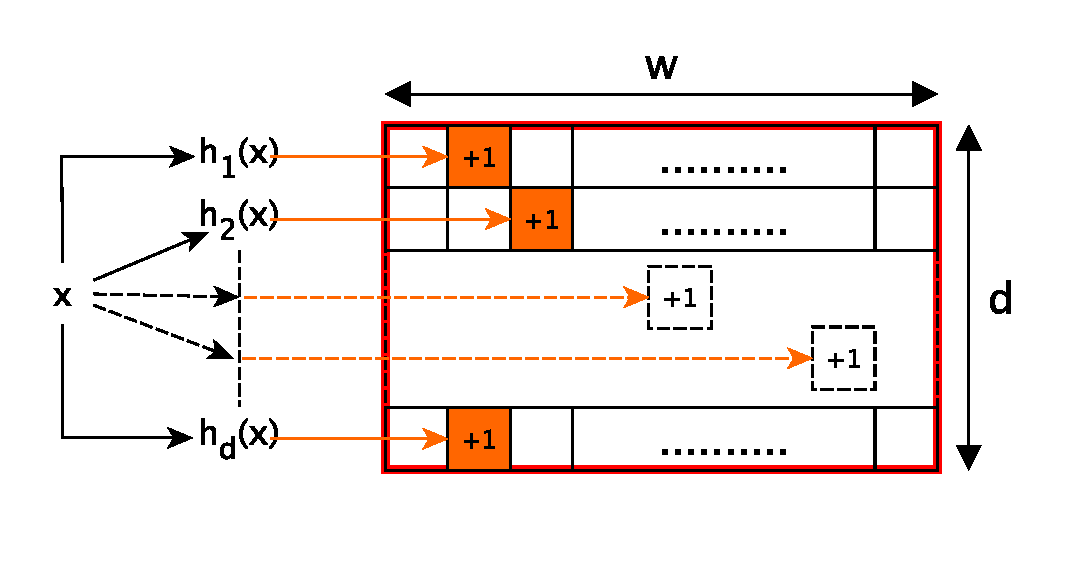
\includegraphics[width=0.90\linewidth]{cms.pdf}
\caption{Illustration of the insert operation for Count-Min Sketch.}
\label{fig:cms_insert}
\end{center}
\end{figure}
 
 \begin{algorithm}[htbp]
  	\small
  	\caption{\textsc{CMS-Construction}} 
  	\KwIn{  $\epsilon$: error factor\\
	 		\hspace*{6ex} $\delta$: error probability \\
	 	  \hspace*{7ex}${\tt s}[.]$: a stream with $N$ elements from $n$ distinct elements \\ 
		  \hspace*{7ex}$h_i(.)$: pairwise independent hash functions where for \\ 
		  \hspace*{13ex}$1\leq i \leq d$,  $h_i$: $\mathcal{U} \rightarrow \{1,\cdots,w\}$ and $w = \lceil e/\epsilon \rceil$\\}
	 \KwOut{ ${\tt cms}[.][.]$: a $d \times w$ counter sketch where $d = \lceil 1/\delta \rceil$ \\
	 }
	 	\For{$i\leftarrow 1$ \KwTo $d$}{
			\For{$j\leftarrow 1$ \KwTo $w$}{
				${\tt cms}$[i][j] $ \leftarrow 0$
			}
		}
		\For{$i\leftarrow 1$ \KwTo $N$}{
			$x  \leftarrow s[i]$
			\For{$j\leftarrow 1$ \KwTo $d$}{
				 $col \leftarrow h_j(x)$
				${\tt cms}$[j][$col$] $ \leftarrow {\tt cms}$[j][$col$] $ +1$
			}
		}
	\label{alg:cms_construct}
\end{algorithm} 	

 
The second operation for CMS is {\em query}($x$) which estimates the frequency of $x \in \mathcal{U}$ as $$f'_x = min_{1 \leq i \leq d}\{{\tt cms}[i][h_i(x)]\}.$$
\noindent With $d \times w$ memory, the sketch satisfies that
 $f_x \leq f'_x$ and $$\Pr\left(f'_x \geq f_x + \epsilon N\right) \leq \delta.$$ Hence, the error is additive and always one-sided, i.e., the
 estimation is always larger than the actual frequency. Furthermore, for $\epsilon$ and $\delta$ small enough, the amount of the error 
 is also bounded with high probability. Hence, especially for frequent items, i.e., when $f_x$ is large, the ratio of the estimation and the actual frequency approaches to one.  

\subsection{Tabulation Hashing}

CMS uses pairwise independent hash functions to provide the desired properties stated above. There exists a separate hash function for each row of the CMS with a range equal 
to the range of columns. In this work, we use Tabulation Hashing~\cite{zobrist1970} which has been recently analyzed by Patrascu and Thorup et al.~\cite{patrascu2012,thorup2017} and shown to provide  strong  statistical guarantees despite of its simplicity. Furthermore, it has been shown that a slightly more sophisticated version of tabulation hashing is almost as fast as the classic multiply-mod-prime scheme, i.e., $(ax + b) \bmod p$. 

Assuming each element in $\mathcal{U}$ is represented in 32 bits and the desired output is also 32 bits, the tabulation hashing works as follows: first a $4 \times 256$ table is generated and filled with random 32-bit values. Given a 32-bit input $x$, each character, i.e., 8-bit value, of $x$ is used as an index for the corresponding row. Hence, four 32-bit values, one from each row, are extracted from the table. The {\tt XOR} of these 32-bit values are returned as the hash value. The implementation we use in this work is given in Figure~\ref{fig:tabulation_seq}.

\begin{figure}[htbp]
\begin{center}
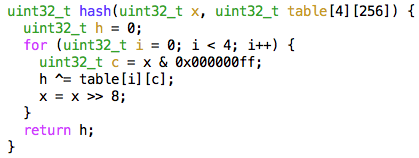
\includegraphics[width=0.90\linewidth]{tabular_code.png}
\caption{Naive tabulation hashing in C++}
\label{fig:tabulation_seq}
\end{center}
\end{figure}

\section{Multiple Tabulation at Once}\label{sec:tab}
Hashing the same item multiple times is a common technique applied in sketch-based data processing to reduce the error of the estimation. One can use a single row for CMS, i.e., set $d = 1$ and answer the query by reporting the value of the counter corresponding to the hash value. However, using multiple rows reduces the probability of having large estimation errors. 

Although the auxiliary data used in tabulation hashing are usually small and can fit into a cache, the spatial locality of the accessed table elements, i.e., the distance among them in memory, is not good enough since each access is performed to a different table row. A naive, cache-friendly rearrangement of the entries in the tables is also not possible for applications performing a single hash per item; the indices for the table rows are obtained from adjacent chunks in the binary representation of the hashed item which are usually not correlated. Hence, there is no relation whatsoever among them to help us to fix the access pattern for all possible stream elements.

In addition to CMS, for many frequency sketches, e.g., Count Sketch~\cite{charikar2002} and Count-Mean-Min Sketch~\cite{Goyal2012}, the same item is hashed more than once. For tabulation hashing, this yields an interesting optimization; there exist multiple hash functions and hence, more than one hash table. Although, the entries in a single table is still accessed in a somehow irregular fashion, the accessed coordinates in all the tables are the same for different tables. This can be observed on the left side of Figure~\ref{fig:merged_tabular_access}. Hence, the columns of the tables can be combined in an alternating fashion as shown in the right side of the figure. In this approach, when only a single thread is responsible from computing the hash values for a single item to CMS, the cache can be utilized in a better way since the memory locations accessed by that thread are adjacent. Hence, the computation will pay the penalty for a cache-miss only once for each 8-bit character of a 32-bit item. This proposed scheme is called {\em merged tabulation}.

 \begin{figure}[htbp]
\begin{center}
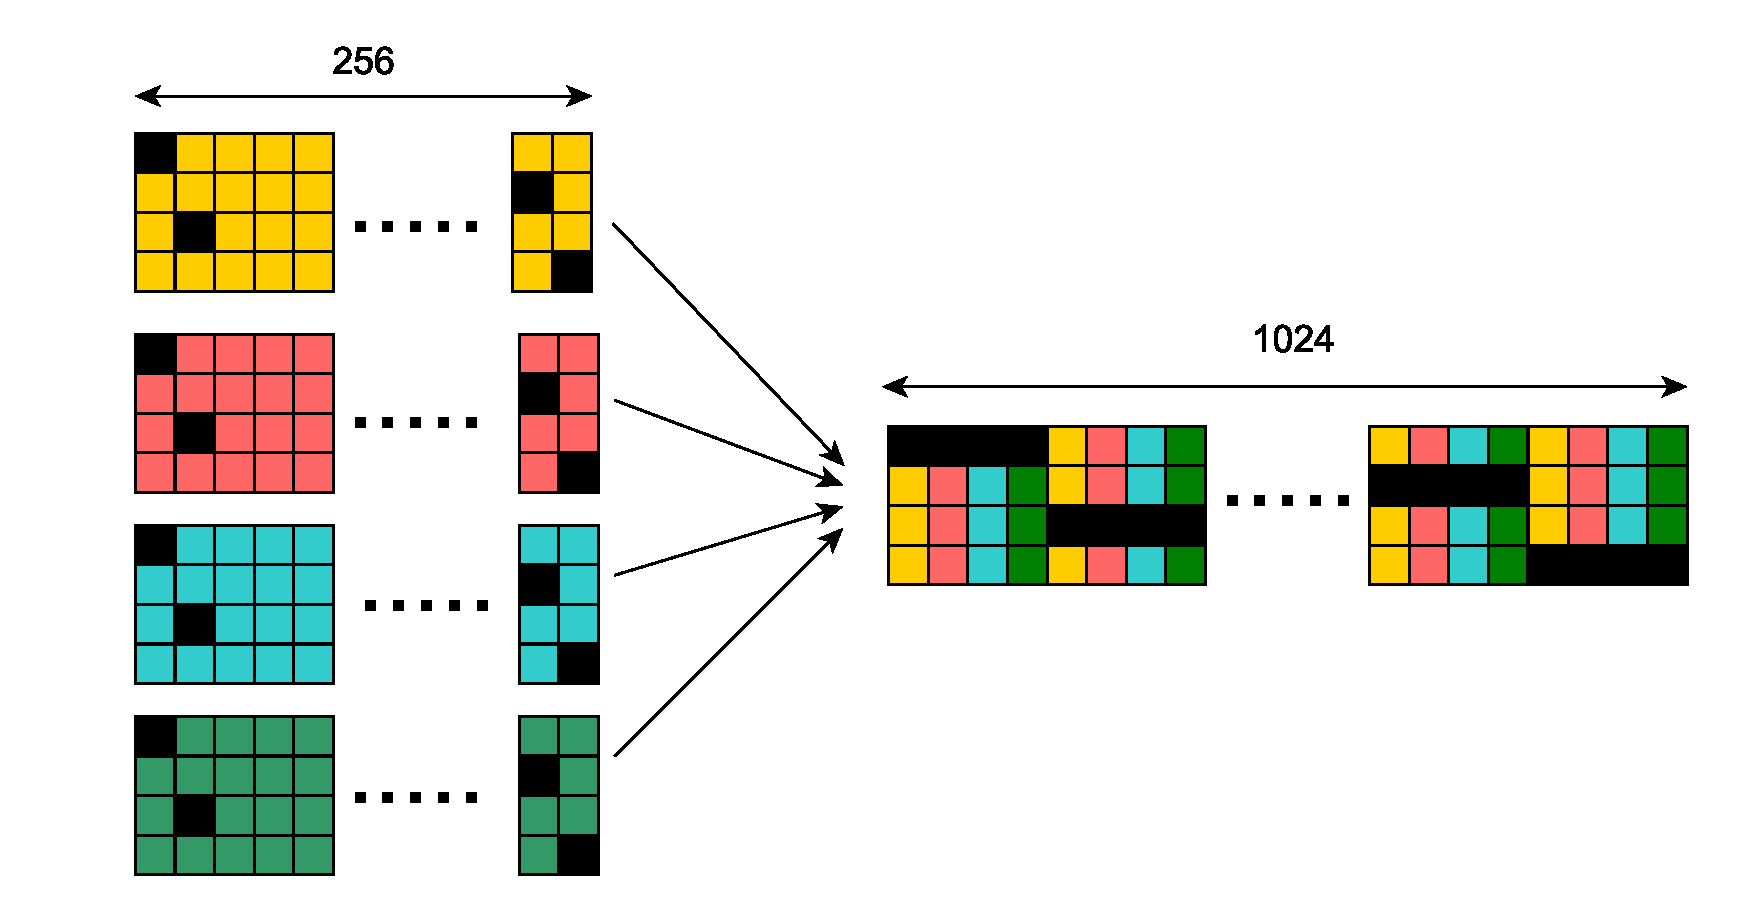
\includegraphics[width=0.96\linewidth]{merged_tabular_access.pdf}
\caption{Memory access patterns for naive and merged tabulation for four hashes. The hash tables are colored with different colors. The accessed locations for both approaches are shown in black.}
\label{fig:merged_tabular_access}
\end{center}
\end{figure}

With merged tabulation, the consecutive elements in the merged table belong to different hash values. Since these values require multiple {\tt XOR} operations, we need to store the partial results in the memory. A simple C++ implementation of merged tabulation which uses a single $4 \times 1024$ table to compute four hashes at once is given in Figure~\ref{fig:tabulation_merged}. We provide actual implementations here for clarity as well as reproducibility.

\begin{figure}[htbp]
\begin{center}
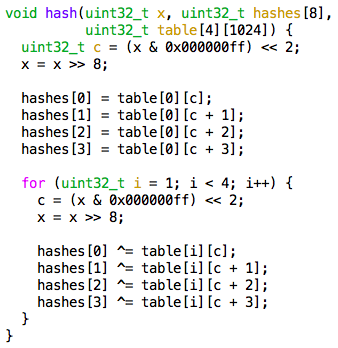
\includegraphics[width=0.70\linewidth]{tabular_code_par}
\caption{Merged tabulation hashing  in C++.}
\label{fig:tabulation_merged}
\end{center}
\end{figure}

\section{Parallel Count-Min Sketch Construction}\label{sec:par}

Since multiple CMS sketches can be combined, on a multicore hardware, each thread can process a different part of the data (with the same hash functions) to construct a partial CMS. These partial sketches can then be aggregated by adding the counter values in the same locations to obtain the final value on the combined CMS sketch. Although this approach has been already proposed in the literature and requires no synchronization until all partial sketches are constructed, compared to constructing the final CMS table directly, it consumes more memory. Furthermore, with this straightforward parallelization, the amount of the memory is increasing with increasing number of threads. Hence, the multi-sketch approach is not scalable.

Constructing a single CMS sketch in parallel is not a straightforward task. The naive approach is assigning each item in the stream to a single thread and let it do the updates (i.e., increment operations) on CMS counters. The pseudocode of this parallel CMS construction is given in Algorithm~\ref{alg:cms_construct_par_nobuf}. However, to compute the counter values correctly, the approach presented in Algorithm~\ref{alg:cms_construct_par_nobuf} requires a significant synchronization overhead; when a thread processes a single data item, it accesses an arbitrary column of each CMS row. Hence, race conditions may reduce the estimation accuracy. In addition, these memory accesses are probable causes of false sharing which prevents the implementation to utilize the hardware to its full potential. To avoid the pitfalls stated above, one can allocate locks on the counters before every increment operation. However, this lock-based manual synchronization is too costly to be applied in practice. 

As an alternative approach, one can assign each item to multiple threads which evaluate different hash functions hence touch different rows of the CMS table. However, this approach cannot use the merged tabulation described in the previous section since, each thread performs only a single hash of an item. 


 \begin{algorithm}[htbp]
  	\small
  	\caption{\textsc{Naive-Parallel-CMS}} 
  	\SetAlgoNoLine
  	\KwIn{  $\epsilon$: error factor\\
	 		\hspace*{6ex} $\delta$: error probability \\
	 	  \hspace*{7ex}${\tt s}[.]$: a stream with $N$ elements from $n$ distinct elements \\ 
		  \hspace*{7ex}$h_i(.)$: pairwise independent hash functions where for \\ 
		  \hspace*{13ex}$1\leq i \leq d$,  $h_i$: $\mathcal{U} \rightarrow \{1,\cdots,w\}$ and $w = \lceil e/\epsilon \rceil$\\
		  \hspace*{7ex}$\tau$: no threads\\ }
	 \KwOut{ ${\tt cms}[.][.]$: a $d \times w$ counter sketch where $d = \lceil 1/\delta \rceil$ \\
	 }
		Reset all the ${\tt cms}[.][.]$ counters to 0 (as in Algorithm~\ref{alg:cms_construct}).
		%\State{}
		
		\For{$i\leftarrow 1$ \KwTo $N$ {\bf in parallel}}{
			$x  \leftarrow s[i]$
			${\tt hashes}[.] \leftarrow$ {\sc MergedHash}($x$)

			\For{$j\leftarrow 1$ \KwTo $d$}{
				$col \leftarrow {\tt hashes}[j] $ 
				${\tt cms}$[j][$col$] $ \leftarrow {\tt cms}$[j][$col$] $ +1$
			}
		}
	\label{alg:cms_construct_par_nobuf}
\end{algorithm} 	

In this work, we propose a {\em buffered parallel} execution to alleviate the above mentioned issues; we (1) divide the data into batches and (2) process a single batch in parallel in two phases; a) multi-hashing and b) CMS counter updates. In the proposed approach, after each batch, the threads synchronize and process the next one. For batches with $b$ elements, the first phase requires a buffer of size $b \times d$ to store the hash values, i.e., column ids, which then will be used in the second phase to update corresponding CMS counters. Such a buffer allows us to use merged tabulation effectively during the first phase. In our implementation, the counters in a row are updated by the same thread hence, there will be no race conditions and probably much less false sharing. We also experiment with extra padding between the table rows which we found to be useful on a server~(but not SBCs), especially for CMS tables with a small $w$ value. Algorithm~\ref{alg:cms_construct_par} gives the pseudocode of the proposed buffered CMS construction approach. 

 \begin{algorithm}[htbp]
  	\small
  	\caption{\textsc{Buffered-Parallel-CMS}} 
  	\KwIn{  $\epsilon$: error factor\\
	 	  \hspace*{6ex} $\delta$: error probability \\
	 	  \hspace*{7ex}${\tt s}[.]$: a stream with $N$ elements from $n$ distinct elements \\ 
		  \hspace*{7ex}$h_i(.)$: pairwise independent hash functions where for \\ 
		  \hspace*{13ex}$1\leq i \leq d$,  $h_i$: $\mathcal{U} \rightarrow \{1,\cdots,w\}$ and $w = \lceil e/\epsilon \rceil$\\
		  \hspace*{7ex}$b$: batch size (assumption: divides $N$)\\
		  \hspace*{7ex}$\tau$: no threads (assumption: divides $d$)\\ }
	 \KwOut{ ${\tt cms}[.][.]$: a $d \times w$ counter sketch where $d = \lceil 1/\delta \rceil$ \\
	 }
		Reset all the ${\tt cms}[.][.]$ counters to 0 (as in Algorithm~\ref{alg:cms_construct})\\[5pt]
		%\State{}
		
		\For{$i\leftarrow 1$ \KwTo $N/b$}{
			$j_{end} \leftarrow i \times b$	 %\Comment{\bf Stage 1}
			$j_{start} \leftarrow j_{end} - b + 1$
			
			\For{$j\leftarrow j_{start}$ \KwTo $j_{end}$ {\bf in parallel}}{
				$x  \leftarrow {\tt s}[j]$
				$\ell_{end} \leftarrow j \times d$
				$\ell_{start} \leftarrow \ell_{end} - d + 1$
				${\tt buf}[\ell_{start}, \cdots, \ell_{end}] \leftarrow$ {\sc MergedHash}($x$)
			}
			
			{{\bf Synchronize} the threads, e.g., with a {\em barrier}}
			
			\For{$t_{id}\leftarrow 1$ \KwTo $\tau$ {\bf in parallel}}{% \Comment{\bf Stage 2}
				\For{$j\leftarrow 1$ \KwTo $b$ }{
					$nrows \leftarrow d / \tau$
					$r_{end} \leftarrow t_{id} \times nrows$
					$r_{start} \leftarrow r_{end} - nrows + 1$
					\For{$r\leftarrow r_{start}$ \KwTo $r_{end}$ }{
						$col \leftarrow {\tt buf}[((j-1) \times d) + r]$
						${\tt cms}[r][col] \leftarrow {\tt cms}[r][col] +1$
			}
			}
			}

			}
	\label{alg:cms_construct_par}
\end{algorithm} 	

\section{Managing Heterogeneous Cores} \label{sec:load}

A recent trend on SBC design is heterogeneous multiprocessing which had been widely adopted by mobile devices. Recently, some ARM-based devices including SBCs use the {\em big.LITTLE} architecture equipped with power hungry but faster cores, as well as battery-saving but slower cores. The faster cores are suitable for compute-intensive, time-critical tasks where the slower ones perform the rest of the tasks and save more energy. In addition, tasks can be dynamically swapped between these cores on the fly. One of the SBCs we experiment in this study has an 8-core Exynos 5422 Cortex processor having four fast and four relatively slow cores. 

Assume that we have $d$ rows in CMS and $d$ cores on the processor; when the cores are homogeneous, Algorithm~\ref{alg:cms_construct_par} works efficiently with static scheduling since, each thread performs the same amount of merged hashes and counter updates. When the cores are heterogeneous, the first inner loop (for merged hashing) can be dynamically  scheduled: that is the batch can be divided into smaller chunks and these chunks can be dynamically assigned to the threads on the fly resulting faster cores seamlessly hash more items. However, {\em dynamic scheduling} will incur a runtime overhead. Furthermore, the same technique is not applicable to the second inner loop where the counter updates are performed: in the proposed buffered approach, Algorithm~\ref{alg:cms_construct_par} divides the workload among the threads by assigning each row to a different one. When the fast cores are done with the updates, the slow cores will still be working. Furthermore, faster cores cannot help to the slower ones by stealing a portion of their remaining jobs since when two threads work on the same CMS row, race conditions will yield more errors on the final counter values. 

To alleviate these problems, we propose to pair a slow core with a fast one. In this approach, each core pair is responsible from two rows where the batch is processed in two stages as shown in Figure~\ref{fig:fastslow}. In the first stage, the items on the batch are processed in a way that the threads running on faster cores update the counters on even numbered CMS rows whereas the ones running on slower cores update the counters on odd numbered CMS rows. When the first stage is done, the thread/core pairs exchange their row ids and resume from the item their mate stopped in the first stage. In both stages, the faster threads process $fastBatchSize$ items and the slower ones process $slowBatchSize$ items where $b = fastBatchSize + slowBatchSize.$

\begin{figure}[htbp]
\begin{center}
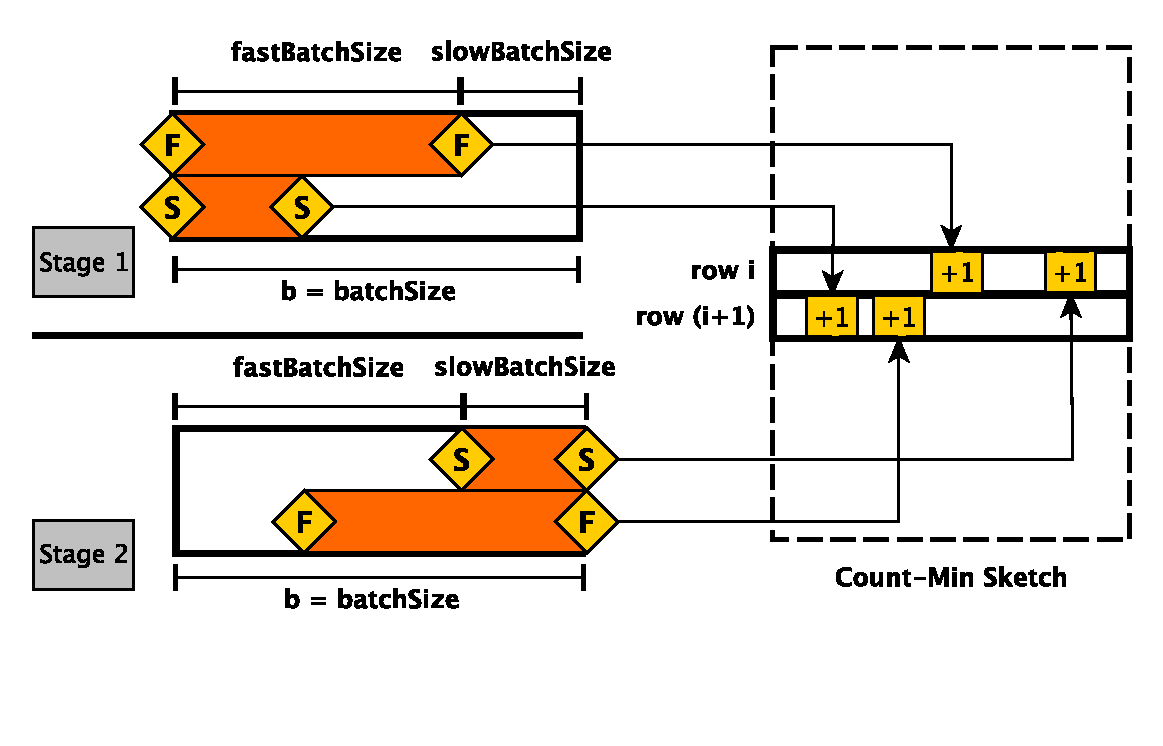
\includegraphics[width=1.03\linewidth]{expfigs/fastslow.pdf}
\caption{For a single batch, rows $i$ and $i+1$ of CMS are updated by a fast and a slow core pair in two stages. In the first stage, the fast core performs row $i$ updates and the slow core processes row $i+1$ updates. In the second stage, they exchange the rows and complete the remaining updates on the counters for the current batch.}
\label{fig:fastslow}
\end{center}
\end{figure}

To avoid the overhead of dynamic scheduling and propose a generic solution, we start with $fastBatchSize = b/2$ and $slowBatchSize = b/2$ and by measuring the time spent by the cores, we dynamically adjust them to distribute the workload among all the cores as fairly as possible. Let $t_F$ and $t_S$ be the times spent by a fast and slow core, respectively, on average. Let $$s_F = \frac{fastBatchSize}{t_F} {\mbox{ \ \ \ \ and \ \ \ }} s_S = \frac{slowBatchSize}{t_S}$$ be the speed of these cores for the same operation, e.g., hashing, CMS update etc. We then solve the equation $$\frac{fastBatchSize + x}{s_F} = \frac{slowBatchSize - x}{s_S}$$ for $x$ and update the values as 
\begin{align*}
fastBatchSize &= fastBatchSize + x\\
slowBatchSize &= slowBatchSize - x
\end{align*}
for the next batch. One can apply this method iteratively for a few batches and use the final values or their average to obtain a generic and dynamic solution for such computations. In this study, we applied this technique both for hashing and counter update phases of the proposed buffered CMS generation algorithm, i.e., for both of the inner loops in Algorithm~\ref{alg:cms_construct_par}. 

\section{Experimental Results}\label{sec:exp}

To understand the performance of the proposed approach, we perform the experiments on three architectures: 
\begin{itemize}[leftmargin=*]
\item {\bf Arch-1} is a server running on 64 bit CentOS 6.5 equipped with 64GB RAM and a dual-socket Intel Xeon E7-4870 v2 clocked at 2.30 GHz where each socket has 15 cores~(30 in total). Each core has a 32KB L1 and a 256KB L2 cache, and each socket has a 30MB L3 cache. 
\item {\bf Arch-2} (Raspberry Pi 3 Model B+) is a quad-core 64-bit ARM Cortex A-53 clocked at 1.4 GHz equipped with 1 GB LPDDR2-900 SDRAM.  Each core has a 32KB L1 cache, and the shared L2 cache size is 512KB.
\item {\bf Arch-3} (Odroid XU4) is an octa-core heterogeneous multi-processor. There are four A15 cores running on 2Ghz and four A7 cores running on 1.4Ghz. The SBC is equipped with a 2GB LPDDR3 RAM. Each core has a 32KB L1 cache. The fast cores have a shared 2MB L2 cache and slow cores have a shared 512KB L2 cache. 
\end{itemize}
For the multicore implementations, we use C++11 and OpenMP. We use {\tt gcc 5.3.0} with the {\tt -O3} optimization flag enabled on {\bf Arch-1}. On {\bf Arch-2}. the compiler is {\tt gcc 6.3.0}, and on {\bf Arch-3}, the compiler is {\tt gcc 7.3.0}. For both SBCs, {\tt -O3} optimization flag is also enabled.

To generate the datasets used in the experiments, we used a {\em Zipfian} distribution~\cite{Zipf1935}. Although this study mainly focuses on the performance which is not directly related to the distribution of the values in the stream ${\tt s}[.]$, many data in real world such as number of paper citations, file transfer sizes, word frequencies etc. fit to a Zipfian distribution. Furthermore, although the error analysis for CMS do not depend on the data, Zipfian is a common choice for the studies in the literature to benchmark the estimation accuracy of data sketches. For completeness and to cover the real-life datasets better, we used the shape parameter $\alpha \in \{1.1, 1.5, 3.0\}$ to understand how the performance of our parallel CMS construction algorithm changes when the distribution of the items, i.e., the variance on the frequencies, change. Note that when the variance between
the item frequencies increase, i.e., when the frequent items become more dominant in the stream, some counters are touched much more than the others. This happens with increasing $\alpha$ and is expected to increase the performance since most of the times, the counters will already be in the cache. To see the other end of the spectrum, in addition to {\em Zipfian}, we also used {\em Uniform} distribution to measure the performance where all counters are expected to be touched the same number of times. 

We employ two sets of $(\epsilon, \delta)$ values to generate CMS tables; in the first one, we used $(\epsilon = 0.01, \delta = 0.004)$ to generate a {\bf small} sketch with $d = \lceil \log_2(1/\delta) \rceil = 8$ and $w = 211$ where $w$ is selected as the first prime after $2/\epsilon$. In addition, we generate a relatively {\bf large} sketch with $(\epsilon = 0.001, \delta = 0.004)$ with $d = 8$ rows and $w = 2003$ columns.

For the experiments on {\bf Arch-1}, we choose $N = 2^{30}$ elements from a universal set $\mathcal{U}$ of cardinality $n = 2^{25}$. For {\bf Arch-2} and   {\bf Arch-3}, we use $N = 2^{25}$ and $n = 2^{20}$. For all architectures, we used $b = 1024$ as the batch size. Each data point in the tables and charts given below is obtained by averaging ten runs. 

\subsection{Parallel CMS construction with partial sketches}

In the first set of experiments, we measure the performance improvement due to merged tabulation in the partial sketches setting. That is, each thread is responsible from a different part of the stream and construct a partial sketch for that part. As mentioned before, this approach consumes more memory and its memory consumption is proportional to the number of threads used. Yet, no synchronization mechanism is required since all the CMS constructions are independent from each other. The results of this set of experiments are given in Table~\ref{tbl:mergedtbl}. 

\begin{table*}[htbp]
\centering
{\def\arraystretch{1}
\begin{tabular}{ccccc||rrrrr|rrrrr}  
                                 &&&&                 & \multicolumn{5}{c|}{\textbf{Naive Tabulation}} & \multicolumn{5}{c}{\textbf{Merged Tabulation}} \\
                                   &&&&                 & $\tau$=1   & $\tau$=2    & $\tau$=4    & $\tau$=8    & $\tau$=16  & $\tau$=1   & $\tau$=2   & $\tau$=4   & $\tau$=8   & $\tau$=16 \\ \hline
                                   
\multicolumn{1}{l}{\multirow{6}{*}{{\rotatebox[origin=c]{90}{\textbf{Uniform}}}}}
&&&\multirow{2}{*}{\textbf{Arch-1}} & \textbf{small}  & 64.3    & 33.1   & 23.1   & 14.0   & 7.6   & 60.4    & 34.4    & 17.5   & 10.0   & 5.2   \\
&&&& \textbf{large} & 72.3    & 36.8   & 20.0   &   9.8 & 4.9   &  60.6 &	33.3 &	17.1	& 8.8	& 4.5 \\ \cline{4-15}

&&&\multirow{2}{*}{\textbf{Arch-2}} & \textbf{small}  & 31.8    & 16.0   & 8.0   &        &       &  28.3    &  14.2   & 7.1   &        &       \\
&&&& \textbf{large} &  33.2      &   16.7     &       8.4 &        &       &     30.8    &     15.4    &     7.8   &        &   \\ \cline{4-15}

&&&\multirow{2}{*}{\textbf{Arch-3}} & \textbf{small}  & 22.7    & 11.4   & 5.9   &   3.4     &       &  21.8    &  10.9   & 5.6   &  3.2      &       \\
&&&& \textbf{large} &  21.5    &  10.9    & 5.6  & 3.5       &       &   20.2    &   10.2   &   5.3   &   3.1     &   \\
\hline    
\hline

%\multicolumn{1}{l}{\multirow{6}{*}{\textbf{Zipf 0.9}}}
%&&&\multirow{2}{*}{\textbf{Arch-1}} & \textbf{small}  & 63.9    & 40.8   & 25.4   & %14.4   & 7.5   & 61.1    & 34.0    & 17.4   & 9.5   & 5.1   \\
%                                 &&&& \textbf{large} & 67.6    & 34.1   & 19.2   &   %9.5 & 4.9   &  60.4 &	33.7 &	17.3	& 8.9	& 4.4 \\ \cline{4-15}
%             
%&&&\multirow{2}{*}{\textbf{Arch-2}} & \textbf{small}  & 31.6    & 15.9   & 8.2   %&        &       &  28.6    &  14.3   & 7.3   &        &       \\
%                                 &&&& \textbf{large} &  32.8      &   16.5     &       %8.3 &        &       &     30.8    &     15.4    &     7.7   &        &   \\ %\cline{4-15}
%                                 
%&&&\multirow{2}{*}{\textbf{Arch-3}} & \textbf{small}  & 22.9    & 11.5   & 5.9   & %3.4   &    & 21.9    & 10.9    & 5.6   & 3.3   &    \\
%&&&& \textbf{large} &  21.5   & 10.9  &  5.6  &  3.5 &    &  20.2 &	10.2 & 5.3	& %3.2	&  \\                                 
%                                  \hline  
\multicolumn{1}{l}{\multirow{6}{*}{{\rotatebox[origin=c]{90}{\textbf{Zipf 1.1}}}}}
&&&\multirow{2}{*}{\textbf{Arch-1}} & \textbf{small}  & 65.8    & 32.2   & 19.6   & 11.9   & 6.1   & 60.0    & 33.1    & 16.6   & 9.0   & 4.8   \\
&&&& \textbf{large} & 65.7    & 33.2   & 18.4   &   9.4 & 4.6   &  60.0 &	32.5 &	16.8	& 8.4	& 4.2 \\ \cline{4-15}

&&&\multirow{2}{*}{\textbf{Arch-2}} & \textbf{small}  & 31.5    & 15.9   & 8.4   &        &       &  28.8    &  14.6   & 7.5   &        &       \\
&&&& \textbf{large} &  32.4      &   16.1     &       10.1 &        &       &     29.6    &     15.0    &     8.9   &        &   \\ \cline{4-15}

&&&\multirow{2}{*}{\textbf{Arch-3}} & \textbf{small}  & 22.7    & 11.4   & 5.9   & 3.4   &    & 21.8    & 10.9    & 5.6   & 3.3   &    \\
&&&& \textbf{large} &  21.3 & 10.8  &  5.5  &  3.4 &    &  20.2 & 10.1 & 5.2	& 3.2	&  \\                                 

\hline 
\multicolumn{1}{l}{\multirow{6}{*}{{\rotatebox[origin=c]{90}{\textbf{Zipf 1.5}}}}}
&&&\multirow{2}{*}{\textbf{Arch-1}} & \textbf{small}  & 63.2    & 32.7   & 17.8   & 10.6   & 5.7   & 59.7    & 30.7    & 15.4   & 7.9   & 4.0   \\
&&&& \textbf{large} & 63.8    & 32.0   & 16.3   &   8.2 & 4.1   &  59.7 &	30.3 &	15.3	& 7.6	& 3.8 \\ \cline{4-15}

&&&\multirow{2}{*}{\textbf{Arch-2}} & \textbf{small}  & 31.1    & 15.7   & 8.0   &        &       &  28.6    &  14.4   & 7.4   &        &       \\
&&&& \textbf{large} &  30.9      &   15.5     &      7.8 &        &       &     28.3    &     14.3    &     7.2   &        &   \\ \cline{4-15}

&&&\multirow{2}{*}{\textbf{Arch-3}} & \textbf{small}  & 22.5    & 11.4   & 5.8   & 3.4   &    & 21.9    & 10.9    & 5.6   & 3.3   &    \\
&&&& \textbf{large} &  20.9	 & 10.6  &  5.4  &  3.3 &    &  20.1 & 10.1 & 5.2	& 3.2	&  \\                   

\hline   
%\multicolumn{1}{l}{\multirow{6}{*}{\textbf{Zipf 2}}}
%&&&\multirow{2}{*}{\textbf{Arch-1}} & \textbf{small}  & 67.8    & 32.8   & 17.1   & 9.1   & 4.3   & 59.8    & 30.3    & 15.1   & 7.7   & 3.9   \\
%&&&& \textbf{large} & 63.0    & 31.6   & 16.0   &  7.9 & 4.0   &  59.8 &	30.0&	15.0	& 7.5	& 3.7 \\ \cline{4-15}

%&&&\multirow{2}{*}{\textbf{Arch-2}} & \textbf{small}  & 31.1    & 15.6   & 8.5   &        &       &  28.8    &  14.8   & 8.0   &        &       \\
%&&&& \textbf{large} &  31.1      &   15.5     &   9.5 &        &       &     28.2    &     14.3    &     8.9   &        &   \\ \cline{4-15}

%&&&\multirow{2}{*}{\textbf{Arch-3}} & \textbf{small}  & 22.1    & 11.2   & 5.8   & 3.4   &    & 21.5    & 10.8    & 5.6   & 3.3   &    \\
%&&&& \textbf{large} &  20.7 & 10.5  &  5.4  &  3.3 &    &  19.9 & 10.0 & 5.2& 3.1	&  \\                   
%
%\hline

\multicolumn{1}{l}{\multirow{6}{*}{{\rotatebox[origin=c]{90}{\textbf{Zipf 3.0}}}}}
&&&\multirow{2}{*}{\textbf{Arch-1}} & \textbf{small}  & 62.9    & 31.9   & 16.4   & 8.3   & 4.2   & 59.8    & 29.9    & 14.9   & 7.5   & 3.7   \\
&&&& \textbf{large} & 63.0    & 31.5   & 15.7   &  7.9 & 3.9   &  60.0 &	29.9&	15.0	& 7.5	& 3.7 \\ \cline{4-15}

&&&\multirow{2}{*}{\textbf{Arch-2}} & \textbf{small}  & 31.0    & 15.8   & 8.3   &        &       &  28.7    &  14.6   & 7.4   &        &       \\
&&&& \textbf{large} &  31.2      &   15.5     &   9.8 &        &       &    28.4    &     14.4    &     8.9   &        &   \\ \cline{4-15} 

&&&\multirow{2}{*}{\textbf{Arch-3}} & \textbf{small}  & 22.5    & 11.4   & 5.8   & 3.4   &    & 21.9    & 11.0    & 5.6   & 3.3   &    \\
&&&& \textbf{large} &  20.3 & 10.3  &  5.3  &  3.2 &    &  19.8 & 9.9 & 5.0& 3.1	&  \\        

 %\hline  
\end{tabular}
}
\caption{Parallel CMS construction times (in seconds) with naive and merged tabulation for $\tau \in \{1, 2, 4, 8, 16\}$ threads on \textbf{Arch-1},  $\tau \in \{1, 2, 4\}$ threads on \textbf{Arch-2}, and $\tau \in \{1, 2, 4, 8\}$ threads on \textbf{Arch-3}. The stream size for \textbf{Arch-1} is $N = 2^{30}$. For \textbf{Arch-2} and \textbf{Arch-3}, $N$ is set to $2^{25}$. The rows labeled with {\bf small} and {\bf large} denote the $8 \times 211$ and $8 \times 2003$ CMS tables, respectively. For this set of experiments, dynamic scheduling is used to overcome the heterogeneity on \textbf{Arch-3}.} \label{tbl:mergedtbl}

\end{table*}

As the results in Table~\ref{tbl:mergedtbl} show, merged tabulation significantly increases the performance of the CMS construction on both \textbf{Arch-1} and  \textbf{Arch-2} even with extra overhead of managing an auxiliary array, i.e., $\tt hashes[.]$ in Figure~\ref{fig:tabulation_merged}. That is instead of using a single register as in naive tabulation~(Figure~\ref{fig:tabulation_seq}), in merged tabulation, the intermediate hash values are first written to the auxiliary memory. Once all $d$ hashes are computed, they are read back from the memory again. However, these extra reads as well as the hash table accesses are more cache friendly.

The impact of merged tabulation changes for different architectures and for {\bf small} and {\bf large} sketches. On {\bf Arch-1}, the runtime decreases when the shape parameter $\alpha$ increases. With $\tau = 16$, for large sketches the improvement is in between $6\%$--$10\%$. For small ones, it is in between $14\%$--$46\%$ and the largest improvement is obtained with the uniform distribution where all the counters, as well as the entries of the auxiliary tables are expected to be touched the same number of times. 

Merged tabulation yields significant speedups on {\bf Arch-2}; when $\tau = 4$, for both small and large sketches, the improvement is in between $8\%$--$13\%$. The proposed technique also improves the runtime on {\bf Arch-3} with $\tau = 8$, around $3\%$--$13\%$. However, the improvement is usually less than $5\%$. 

An interesting observation is the relative performances of the architectures on small and large sketches. Considering the cases with $\tau \geq 4$, \textbf{Arch-1} and \textbf{Arch-3} almost always process the stream faster when the sketch is large, i.e., $8 \times 2003$. For \textbf{Arch-1} the difference between the performance reduces with merged tabulation. On the contrary to these architectures, \textbf{Arch-2} processes the stream faster when the sketch is small. We note that this architecture has the least amount of cache available and hence, it suffers more when the memory footprint is large. 

%On {\bf Arch-2}, the improvements on the CMS construction time with $\tau = 1$, $2$ and $4$ threads are $10.5\%$, $11\%$ and $12\%$ on {\bf small} sketches and $6.5\%$, $7\%$ and $8\%$ on {\bf large} sketches, respectively.  Hence, the amount of the improvement does not change with the number of threads and sketch sizes. On {\bf Arch-1}, the improvement starts with $4.5\%$ with a single thread for the {\bf small} sketch, merged tabulation increases the runtime by $2\%$ for two threads., with $\tau = 2$, $4$, $8$ and $16$, the improvement becomes $20\%$, $46\%$, $51\%$ and $47\%$, respectively. On the other hand, for the {\bf large} sketch, the improvement is more stable and in between $2\%$ and $12\%$ for varying number of threads.


\subsection{Parallel CMS construction with a single sketch}

Although using partial sketches is pleasingly parallelizable and can be practical for some use cases, it is not a good approach for memory restricted devices such as SBCs. The additional memory might be required by other applications running on the same hardware and/or other types of skeches being maintained at the same time for the same or a different data stream. 
A straightforward parallelization with multiple sketches uses $(d \times w \times \tau)$ counters
where each counter can have a value as large as $N$. Hence, memory consumption is
$$(d \times w \times \tau \times \log N)$$ bits. On the other hand, a single sketch with buffering
consumes $$(d \times ((w \times \log N) + (b \times \log w)))$$ bits since there are $(d \times b)$ entries in the
buffer and each entry is a column ID on CMS. For instance, with $\tau = 8$ threads, $\epsilon = 0.001$ and $\delta = 0.004)$, the straightforward parallelization with multiple
sketches require $(8 \times 2003 \times 8 \times 30) =$ 3.85Mbits whereas using single sketch requires
$(8 \times ((2003 \times 30) + (1024 \times 11))) =$ 570Kbits. This is why in the rest of the experiments, we focus on the single CMS case. We also keep using merged tabulation.  

Table~\ref{tbl:batch} shows the results of the experiments in which a single sketch is constructed in parallel. As expected, the naive parallel approach~(first set of columns in Table~\ref{tbl:batch}) suffers from false sharing with multiple threads on {\bf Arch-1}. However, we did not observe the such a dramatic slowdown on {\bf Arch-2} and {\bf Arch-3}. We think that the behavior is different since ARM-based processors use a weaker memory consistency model which reduces the impact of race conditions encountered during parallel execution. 

For sequential executions, the proposed buffering technique behaves differently on these architectures; Since storing intermediate hash values has an overhead, we expect a slowdown in a sequential execution. This is what we have observed on {\bf Arch-1}; the runtimes are increased to 67--68 seconds from 60--63 seconds both for small and large sketches. 
However, even with this extra overhead, the technique significantly increases the sequential performance of {\bf Arch-2}, especially for the large sketches. 
Although not as significant as {\bf Arch-2}, buffering yields a slight improvement even for {\bf Arch-3}. 
We believe that the difference is due to the existence of a relatively smaller cache sizes on {\bf Arch-2}. On {\bf Arch-3}, we have a slightly larger cache, and {\bf Arch-1} has the largest cache sizes. In the naive approach, an item is hashed with merged tabulation and then $d$ counters are updated. This process is repeated in an alternating fashion for all the data items in the stream. Hence, the merged hash table and the CMS are accessed one after another which makes these structures alive in the cache at the same time as much as possible which may result cache trashing.  An advantage of buffering is that it separates the accesses to these structures. Hence, it tends not to use the cache for both structures at the same time. Thus for a sequential execution, where the pressure on the cache is low, the overhead of buffering exceeds its benefits for larger cache sizes. On the contrary, it becomes useful for cache-restricted devices such as SBCs even for a sequential execution despite the overhead. 

With multiple threads, the pressure on the cache increases further. In this case, the buffered parallel approach given in Algorithm~\ref{alg:cms_construct_par}~(the second set of columns in Table~\ref{tbl:batch}) is significantly better than the naive parallel one; it improves the runtimes and yields a better scalability. However, on {\bf Arch-1}, the proposed approach yields much less parallel efficiency compared to the other results. This is expected since, with multiple threads performing simultaneous updates on the sketch, false sharing reduces the performance. Furthermore, the impact will be more drastic for smaller sketches which is the case in our experiments. To avoid false sharing as much as possible, we added extra padding to each row of CMS sketch. The third set of columns in Table~\ref{tbl:batch} shows the execution times after padding. As the results confirm, padding helps to get rid of the problems arose from increased coherency traffic due to the concurrent updates on the same cache line by multiple threads. 

\begin{table*}[htbp]
\scalebox{0.95}{
\small
\centering
{\def\arraystretch{1}
\begin{tabular}{ccc||rrrrr|rrrrr|rrrrr}
                                   &&                 & \multicolumn{5}{c|}{\textbf{Naive Parallel}} & \multicolumn{5}{c|}{\textbf{Buffered Parallel}} & \multicolumn{5}{c}{\textbf{Buffered Parallel + P}} \\
                                                                      &&                 & \multicolumn{5}{c|}{(Algorithm~\ref{alg:cms_construct_par_nobuf})} & \multicolumn{5}{c|}{(Algorithm~\ref{alg:cms_construct_par})} & \multicolumn{5}{c}{(Algorithm~\ref{alg:cms_construct_par} + Padding)} \\

                                   &&                 & $\tau$=1   & $\tau$=2    & $\tau$=4    & $\tau$=8    & $\tau$=16  & $\tau$=1   & $\tau$=2   & $\tau$=4   & $\tau$=8   & $\tau$=16  & $\tau$=1   & $\tau$=2   & $\tau$=4   & $\tau$=8   & $\tau$=16 \\ \hline
%\multicolumn{1}{c}{\multirow{8}{*}{\textbf{Zipf 0.9}}} 
%&\multirow{2}{*}{\textbf{Arch-1}} & \textbf{small}  & 61.4  & 289.8  & 287.0  & 176.6  & 118.3 & 68.0  & 61.9  & 45.0  & 29.7  & 27.2  & 68.3  & 46.7  & 24.4    & 13.6  & 10.9 \\
%                                   && \textbf{large} & 60.4  & 240.0  & 225.3  & 137.2  & 96.9  & 68.6  & 50.3  & 28.2  & 15.8& 13.4&68.5&43.6&22.7&12.7& 10.4 \\ \cline{2-18}
%&\multirow{2}{*}{\textbf{Arch-2}}  & \textbf{small}  & 28.7  & 15.4   & 7.7   &        &       & 27.7  & 13.8  & 7.4  &       &       & 27.8  & 13.8  & 7.5  &       &      \\
%                                   && \textbf{large} & 30.7  & 15.4   & 7.7   &        &       & 26.8  & 13.3  & 8.3  &       &       & 27.2  & 13.3  & 8.3  &       &  \\
%                                   \cline{2-18}
                                   
%&\multirow{2}{*}{\textbf{Arch-3 Naive}}  & \textbf{small}  & 22.0  &11.3  &6.0    &5.3    &       & 22.4  & 12.4  & 6.3  & 4.5      &       & 22.4  & 12.4  & 6.2 & 4.5      &      \\
%&& \textbf{large} & 20.3  & 10.4   & 5.4   &  4.9   &       & 21.1  & 11.4  & 5.8  & 4.3      &       & 20.6  & 11.3  & 5.7  & 4.3       &  \\       
%\cline{2-18}

%&\multirow{2}{*}{\textbf{Arch-3 Balanced}}  & \textbf{small}  & 22.0  &11.3    &6.0    &5.3    &       & 21.8  & 12.1  & 6.2  & 3.8      &       & 21.8  & 12.1  & 6.2 & 3.8      &      \\
%&& \textbf{large} & 20.3  & 10.4   & 5.4   &  4.9       &       & 20.6  & 11.1  & 5.7  & 3.6      &       & 20.6  & 11.4  & 5.7  & 3.6       &  \\                                 
                                   
%\hline 
 

\multicolumn{1}{l}{\multirow{8}{*}{{\rotatebox[origin=c]{90}{\textbf{Uniform}}}}}
&\multirow{2}{*}{\textbf{Arch-1}} & \textbf{small}  & 61.5  & 299.9  & 304.4  & 201.7  & 156.9 & 68.3  & 60.9  & 45.5  & 30.4  & 28.0  & 68.6  & 43.5   & 22.8   & 13.0   & 10.6 \\
&& \textbf{large} & 60.1  & 233.8  & 229.2  & 139.2  & 96.5  & 68.7  & 51.4  & 29.8  & 17.1& 14.4&68.8& 45.0   & 23.2   &   13.0 & 10.6  \\ \cline{2-18}
&\multirow{2}{*}{\textbf{Arch-2}}  & \textbf{small}  & 28.5  & 15.4   & 7.8   &        &       & 27.5  & 13.8  & 6.9  &       &       & 27.6  & 13.8  & 6.9  &       &      \\
&& \textbf{large} & 30.8 & 15.4   & 7.7   &        &       & 26.8  & 13.3  & 6.6  &       &       & 26.8  & 13.3  & 6.6  &       &  \\ \cline{2-18}
&\multirow{2}{*}{\textbf{Arch-3}}  & \textbf{small}  & 22.0  & 11.2   & 6.0   &5.3    &       & 21.8  & 12.2  & 6.3  & 4.5	      &       & 21.8  & 12.2& 6.2 & 4.5      &      \\
&& \textbf{large} & 20.3  & 10.3  & 5.5   &  5.1       &       & 20.6  & 11.1  & 5.7  & 4.3      &       & 20.6  & 11.1 & 5.7  & 4.3       &  \\ \cline{2-18}
&\multirow{2}{*}{\textbf{Arch-3++}}  & \textbf{small}  & 22.0  & 11.2   & 6.0   &5.3    &       & 21.8  & 12.2  & 6.3  & 3.9      &       & 21.8  & 12.2& 6.2 & 3.9      &      \\
&& \textbf{large} & 20.3  & 10.3  & 5.5   &  5.1       &       & 20.6  & 11.1  & 5.7  & 3.7      &       & 20.6  & 11.1 & 5.7  & 3.7       &  \\

\hline 
\hline

\multicolumn{1}{l}{\multirow{8}{*}{{\rotatebox[origin=c]{90}{\textbf{Zipf 1.1}}}}}
&\multirow{2}{*}{\textbf{Arch-1}} & \textbf{small}  & 60.3  & 287.6  & 287.3  & 179.3  & 125.9 & 68.1  & 58.4  & 40.1  & 26.2  & 24.1  & 68.1  & 43.5  & 22.9    & 13.0  & 10.6 \\
&& \textbf{large} & 60.9  & 146.1  & 222.2  & 159.1  & 130.5  & 68.3  & 51.4  & 28.7  & 16.0& 13.2&68.4&46.4&24.3&13.6& 10.8 \\ \cline{2-18}
&\multirow{2}{*}{\textbf{Arch-2}}  & \textbf{small}  & 28.7  & 15.5   & 8.6   &        &       & 27.7  & 13.9  & 7.4  &       &       & 27.9  & 13.9  & 7.4  &       &      \\
&& \textbf{large} & 30.2 & 15.4   & 9.5   &        &       & 26.8  & 13.3  & 8.1  &       &       & 27.1  & 13.3  & 8.1  &       &  \\ \cline{2-18}

&\multirow{2}{*}{\textbf{Arch-3}}  & \textbf{small}  & 22.1  &11.3    &6.0    &5.3    &       & 21.7  & 12.1  & 6.2  & 4.5      &       & 21.7  & 12.1  & 6.2 & 4.5      &      \\
&& \textbf{large} & 20.3  & 10.4   & 5.5   &  5.0       &       & 20.4  & 11.1  & 5.7  & 4.3      &       & 20.5  & 11.1  & 5.7  & 4.3       &  \\ \cline{2-18}

 &\multirow{2}{*}{\textbf{Arch-3++}}  & \textbf{small}  & 22.1  &11.3    &6.0    &5.3    &       & 21.7  & 12.1  & 6.2  & 3.8      &       & 21.7  & 12.1  & 6.2 & 3.8      &      \\
 && \textbf{large} & 20.3  & 10.4   & 5.5   &  5.0       &       & 20.4  & 11.1  & 5.7  & 3.6      &       & 20.5  & 11.1  & 5.7  & 3.6       &  \\ 
\hline 

\multicolumn{1}{l}{\multirow{8}{*}{{\rotatebox[origin=c]{90}{\textbf{Zipf 1.5}}}}}
&\multirow{2}{*}{\textbf{Arch-1}} & \textbf{small}  & 62.8  & 331.8  & 314.2  & 206.8  & 166.1 & 68.0  & 53.0  & 34.2  & 20.6  & 18.5  & 68.1  &  44.6   & 23.5   & 13.1   & 10.6   \\
&& \textbf{large} & 63.4  & 214.2  & 257.5  & 193.6  & 170.5  & 68.3  & 47.5  & 25.8  & 14.6& 12.1&68.3&43.7   & 23.1   &   13.0 & 10.5  \\ \cline{2-18}
&\multirow{2}{*}{\textbf{Arch-2}}  & \textbf{small}  & 30.7  & 16.4   & 8.5   &        &       & 27.4  & 13.7  & 6.9  &       &       & 27.3  & 13.7  & 7.0  &       &      \\
&& \textbf{large} & 30.8 & 16.1   & 10.3   &        &       & 26.5  & 13.2  & 7.4  &       &       & 26.5  & 13.2  & 7.5  &       &  \\ \cline{2-18}

&\multirow{2}{*}{\textbf{Arch-3}}  & \textbf{small}  & 22.1  &11.3    &6.0    &5.7    &       & 21.7  & 12.1  & 6.2  & 4.4      &       & 21.7  & 12.1  & 6.2 & 4.4      &      \\
&& \textbf{large} & 20.1  & 10.4   & 5.5   &  5.4       &       & 19.9  & 10.9  & 5.6  & 4.2      &       & 20.0  & 11.0  & 5.6  & 4.3       &  \\  \cline{2-18}  

&\multirow{2}{*}{\textbf{Arch-3++}}  & \textbf{small}  & 22.1  &11.3    &6.0    &5.7    &       & 21.7  & 12.1  & 6.2  & 3.8      &       & 21.7  & 12.1  & 6.2 & 3.8      &      \\
&& \textbf{large} & 20.1  & 10.4   & 5.5   &  5.4       &       & 19.9  & 10.9  & 5.6  & 3.6      &       & 20.0  & 11.0  & 5.6  & 3.5       &  \\     

\hline 

%\multicolumn{1}{c}{\multirow{8}{*}{\textbf{Zipf 2}}} 
%&\multirow{2}{*}{\textbf{Arch-1}} & \textbf{small}  & 62.8  & 340.5  & 330.0  & 236.8  & 207.2 & 67.7  & 49.0  & 27.6  & 15.8  & 14.0  & 67.7  & 44.5  & 23.6    & 13.1  & 10.6 \\
%&& \textbf{large} & 64.6  & 261.7  & 311.0  & 232.3  & 204.3  & 68.0  & 44.5  & 23.6  & 14.9& 12.7&68.0&43.7&23.1&13.7& 10.5 \\ \cline{2-18}
%&\multirow{2}{*}{\textbf{Arch-2}}  & \textbf{small}  & 31.2  & 16.5   & 9.5   &        &       & 27.3  & 13.7  & 7.2  &       &       & 27.4  & 13.7  & 7.2  &       &      \\
%&& \textbf{large} & 31.2 & 16.3   & 10.5   &        &       & 26.2  & 13.0  & 7.9  &       &       & 26.4  & 13.0  & 7.9  &       &  \\ \cline{2-18}

%&\multirow{2}{*}{\textbf{Arch-3 Naive}}  & \textbf{small}  & 21.8  & 11.3   & 6.0   &6.2    &       & 21.7  & 12.1  & 6.1  & 4.4      &       & 22.3  & 12.7 & 6.1 & 4.4      &    \\
%&& \textbf{large} & 20.0  & 10.4  & 5.5   &  6.0       &       & 19.8  & 11.0  & 5.6  & 4.3      &       & 19.7  & 11.0  & 5.5  & 4.2       &  \\ \cline{2-18}

%&\multirow{2}{*}{\textbf{Arch-3 Balanced}}  & \textbf{small}  & 21.8  & 11.3   & 6.0   &6.2    &       & 20.9  & 11.7  & 5.9  & 3.7      &       & 21.0  & 11.7 & 5.9 & 3.7      &      \\
%&& \textbf{large} & 20.0  & 10.4  & 5.5   &  6.0       &       & 19.3  & 10.8  & 5.5  & 3.4      &       & 20.0  & 11.0  & 5.6  & 3.5       &  \\     

%\hline 

\multicolumn{1}{l}{\multirow{8}{*}{{\rotatebox[origin=c]{90}{\textbf{Zipf 3.0}}}}}
&\multirow{2}{*}{\textbf{Arch-1}} & \textbf{small}  & 62.9  & 372.5  & 340.8  & 278.5  & 250.8 & 67.6  & 45.2  & 24.6  & 13.8  & 11.4  & 67.7  & 43.1  & 22.9    & 12.8  & 10.5 \\
&& \textbf{large} & 62.9  & 319.2  & 349.0  & 282.1  & 253.5  & 67.7  & 38.6  & 22.6  & 13.0& 11.0&68.1&44.4&23.1&13.1& 11.2 \\ \cline{2-18}
&\multirow{2}{*}{\textbf{Arch-2}}  & \textbf{small}  & 30.7  & 16.4   & 8.5   &        &       & 27.0  & 13.5  & 7.2  &       &       & 27.3  & 13.7  & 7.2  &       &      \\ 
&& \textbf{large} & 30.8 & 16.1   & 10.3   &        &       & 26.2  & 13.0  & 7.4  &       &       & 26.3  & 13.1  & 7.4  &       &  \\ \cline{2-18}

&\multirow{2}{*}{\textbf{Arch-3}}  & \textbf{small}  & 21.5  & 12.1   & 6.2   &4.4    &       & 21.1  & 11.7  & 6.0  & 4.4      &       & 20.3  & 11.4 & 5.8 & 4.4      &      \\
&& \textbf{large} & 19.7  & 11.2  & 5.8   &  4.3       &       & 18.7  & 10.6  & 5.3  & 4.3      &       & 19.2  & 11.0 & 5.5  & 4.3       &  \\ \cline{2-18}

&\multirow{2}{*}{\textbf{Arch-3++}}  & \textbf{small}  & 21.5  & 12.1   & 6.2   &4.4    &       & 21.1  & 11.7  & 6.0  & 3.6      &       & 20.3  & 11.4& 5.8 & 3.6      &      \\
&& \textbf{large} & 19.7  & 11.2  & 5.8   &  4.3       &       & 18.7  & 10.6  & 5.3  & 3.3      &       & 19.2  & 11.0 & 5.5  & 3.4       &  \\
\end{tabular}
}
}
\caption{Parallel CMS construction times (in seconds) with a single sketch for $\tau \in \{1, 2, 4, 8, 16\}$ threads on \textbf{Arch-1},  $\tau \in \{1, 2, 4\}$ threads on \textbf{Arch-2}, and $\tau \in \{1, 2, 4, 8\}$ threads on \textbf{Arch-3}. \textbf{Arch-3++} represents the approach to take care of the heterogeneity which we only applied for $\tau = 8$. For less number of cores, only fast cores are employed.  The stream size for \textbf{Arch-1} is $N = 2^{30}$. For \textbf{Arch-2} and \textbf{Arch-3}, $N$ is set to $2^{25}$. The rows labeled with {\bf small} and {\bf large} denote the $8 \times 211$ and $8 \times 2003$ CMS tables, respectively.  The {\bf Naive Parallel} construction does not apply buffering or padding whereas the next two sets of columns apply these techniques. For {\bf Buffered Parallel} construction w/out padding, when $\tau = 16$, all threads are utilized for the first phase of Algorithm~\ref{alg:cms_construct_par}, i.e., hashing, but only $d = 8$ of them are used for the second phase.}\label{tbl:batch}
\end{table*}

\subsubsection{Managing heterogeneous cores:} For {\bf Arch-3}, which equipped with a heterogeneous multi-processor, we applied the workload distribution technique described in Section~\ref{sec:load}. We pair each slow core with a fast one, virtually divide each batch into two parts and make the slow core always run on smaller part. 
As mentioned before, for each batch, we dynamically adjust the part sizes based on the previous runtimes of slow and fast cores. Figure~\ref{fig:load} shows the ratio $$F2S = \frac{fastBatchSize}{slowBatchSize}$$ for the first $256$ batches. As expected, the best F2S changes w.r.t. the computation performed; for hashing a 4-to-1 division of workload yields a fair distribution. However, for CMS updates a 1.8-to-1 division is the best one yielding a fair distribution. As the figure shows, the F2S ratio becomes stable after a few batches for both phases. Hence, one can stop the update process after $\thicksim\xspace30$  batches and use a constant F2S for the later ones.

The proposed workload distribution technique improves the runtime on {\bf Arch-3} and increase the parallel efficiency by $15\%$--$30\%$ for $\tau = 8$ threads.   

\begin{figure*}[htbp]
	\begin{subfigure}[t]{0.45\textwidth}
		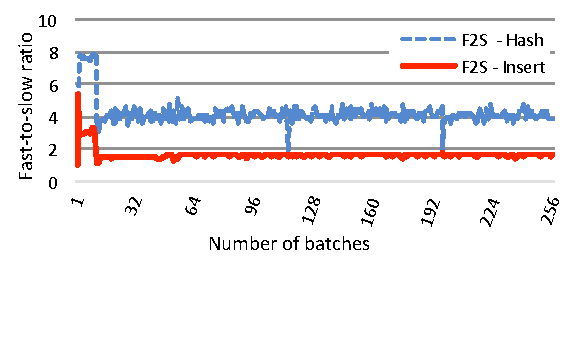
\includegraphics[width=\linewidth]{expfigs/f2s-small.pdf}
		\caption{{\bf small} on {\bf Arch-3++}}
		\label{fig:fs-small}
	\end{subfigure}\hspace*{4ex}
	\begin{subfigure}[t]{0.45\textwidth}
		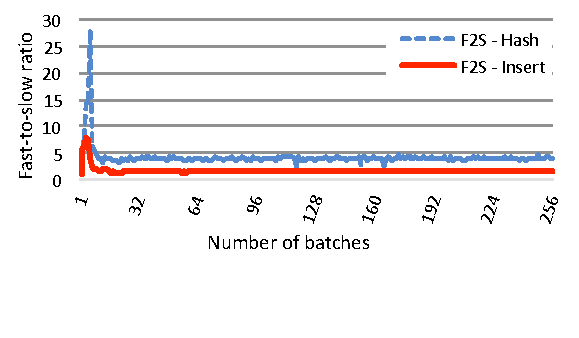
\includegraphics[width=\linewidth]{expfigs/f2s-big.pdf}
		\caption{{\bf large} on {\bf Arch-3++}}
		\label{fig:fs-large}
	\end{subfigure}
	
	\caption{Plots of fast-to-slow ratio $F2S = \frac{fastBatchSize}{slowBatchSize}$ of hashing and CMS update phases for consecutive batches and for small~(left) and large~(right) sketches.}
	\label{fig:load}
\end{figure*}

\subsubsection{Analyzing the time spent for different phases:} Figure~\ref{fig:sum} summarizes all the experiments on parallel construction of a single CMS sketch with individual execution times for the first and the second phases of buffered parallel executions. For all the experiment, the first phase, i.e., hashing phase is takes much less time compared to the second phase, i.e., CMS update phase. An interesting observation is that for almost of all executions, the relative execution time of CMS update phase to whole execution time is much larger for SBCs. We believe that this is due to much faster execution of this phase on \textbf{Arch-1}.



\begin{figure*}[htbp]
\begin{subfigure}[t]{0.43\textwidth}
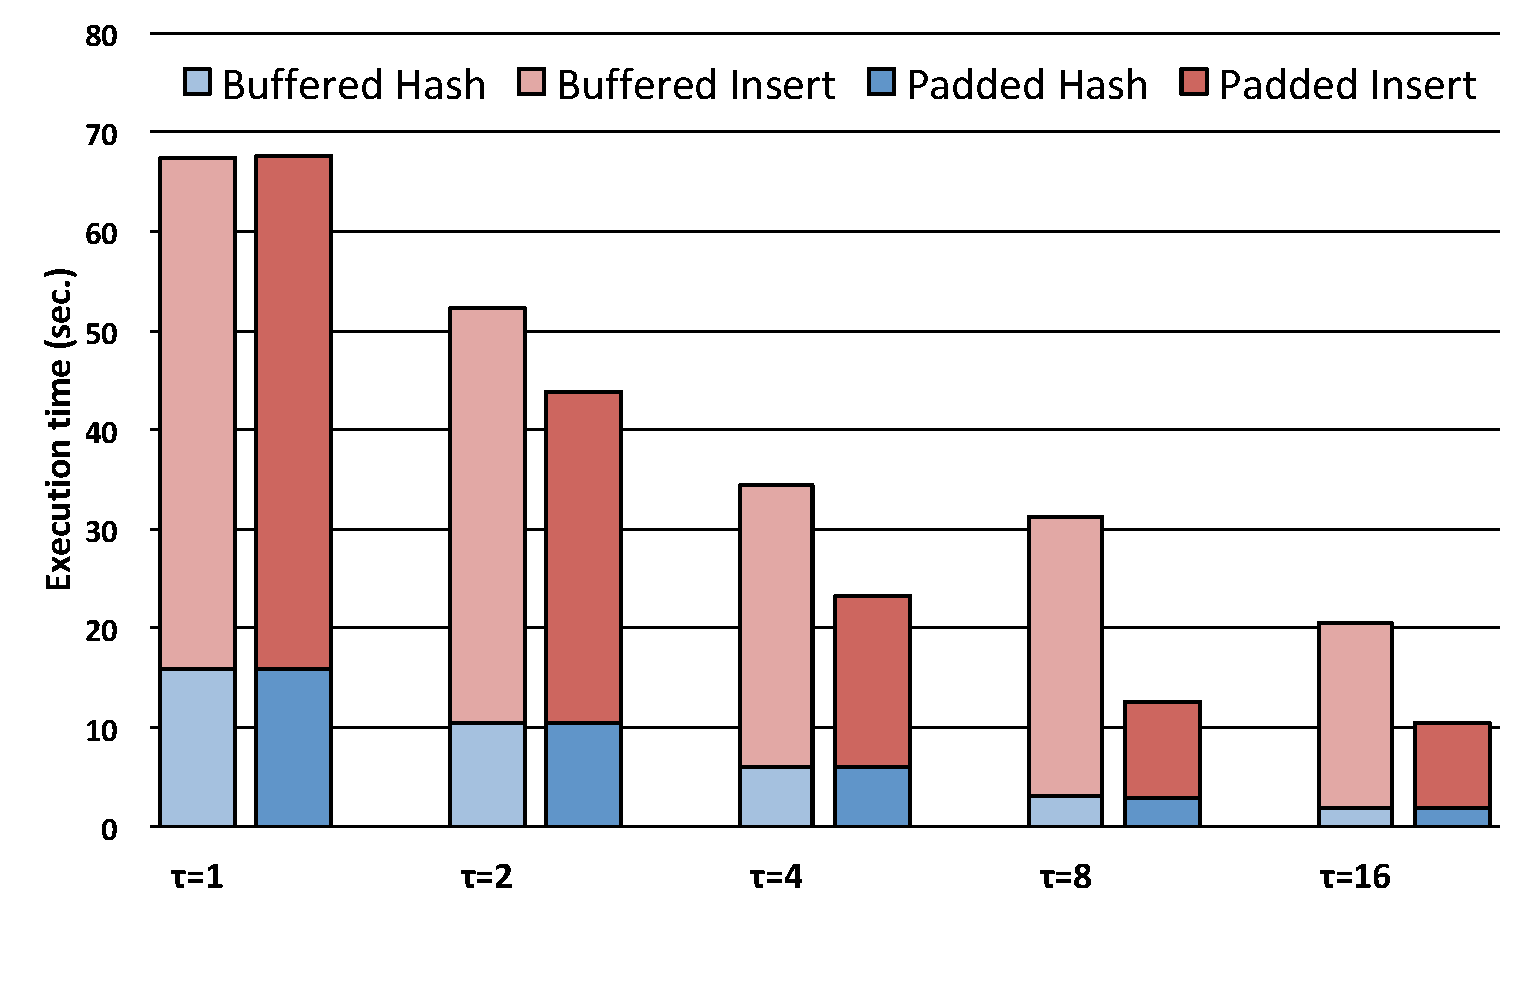
\includegraphics[width=\linewidth]{expfigs/small-gandalf.pdf}
\caption{{\bf small} on {\bf Arch-1}}
\label{fig:8x211arch1}
\end{subfigure}
\begin{subfigure}[t]{0.43\textwidth}
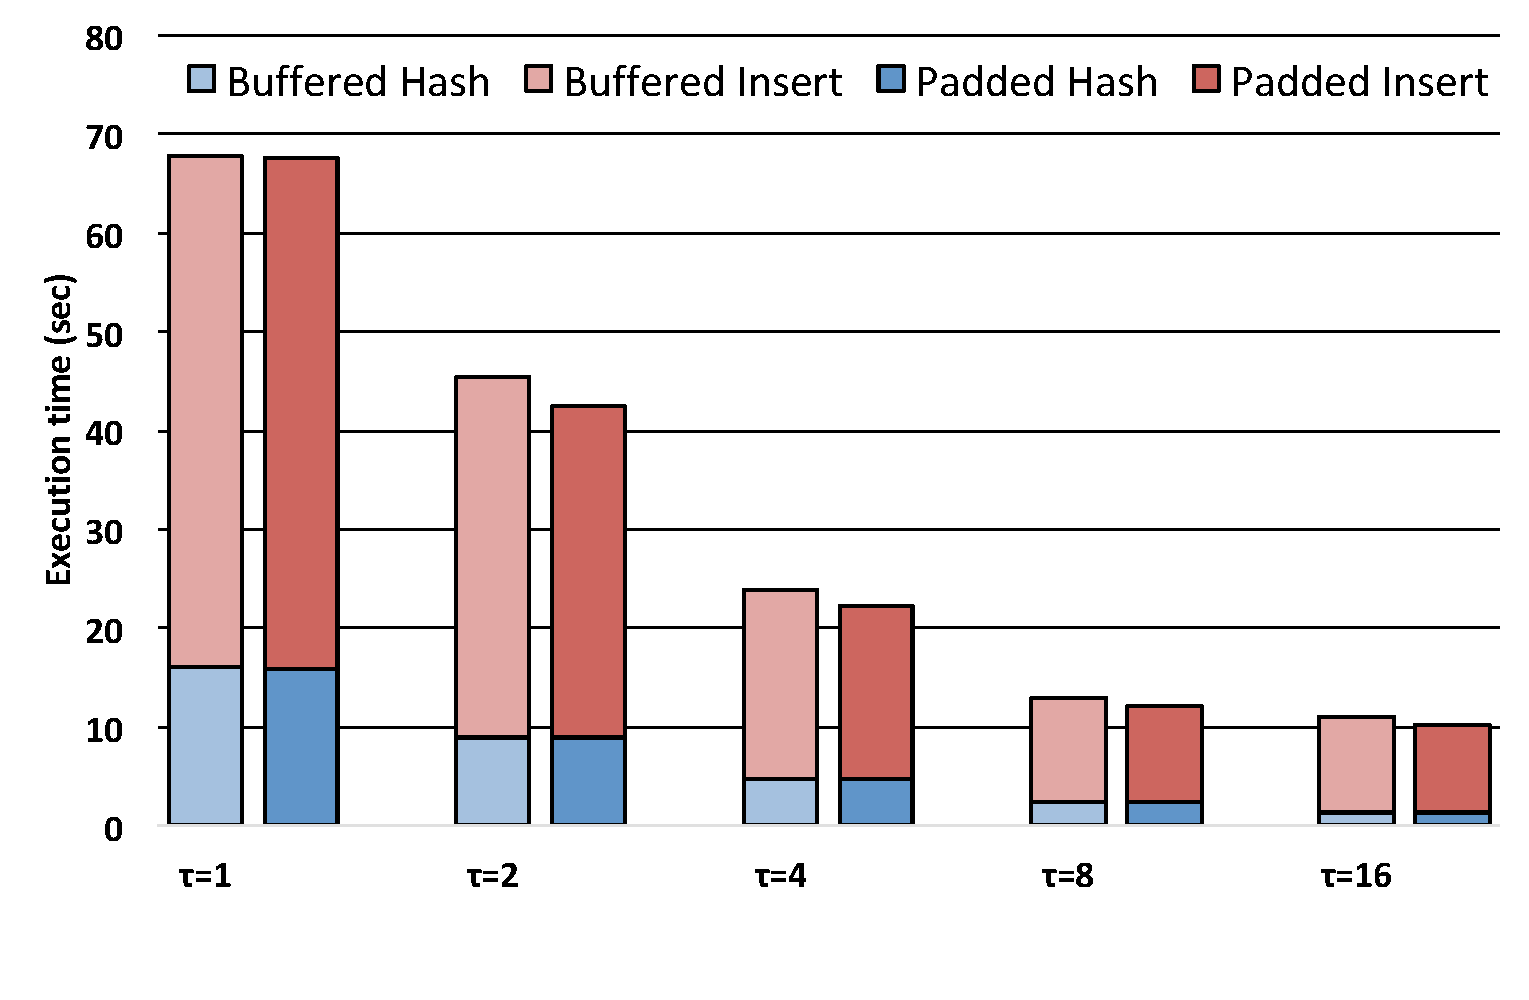
\includegraphics[width=\linewidth]{expfigs/large-gandalf.pdf}
\caption{{\bf large} on {\bf Arch-1}}
\label{fig:8x2003arch1}
\end{subfigure}
\begin{subfigure}[t]{0.43\textwidth}
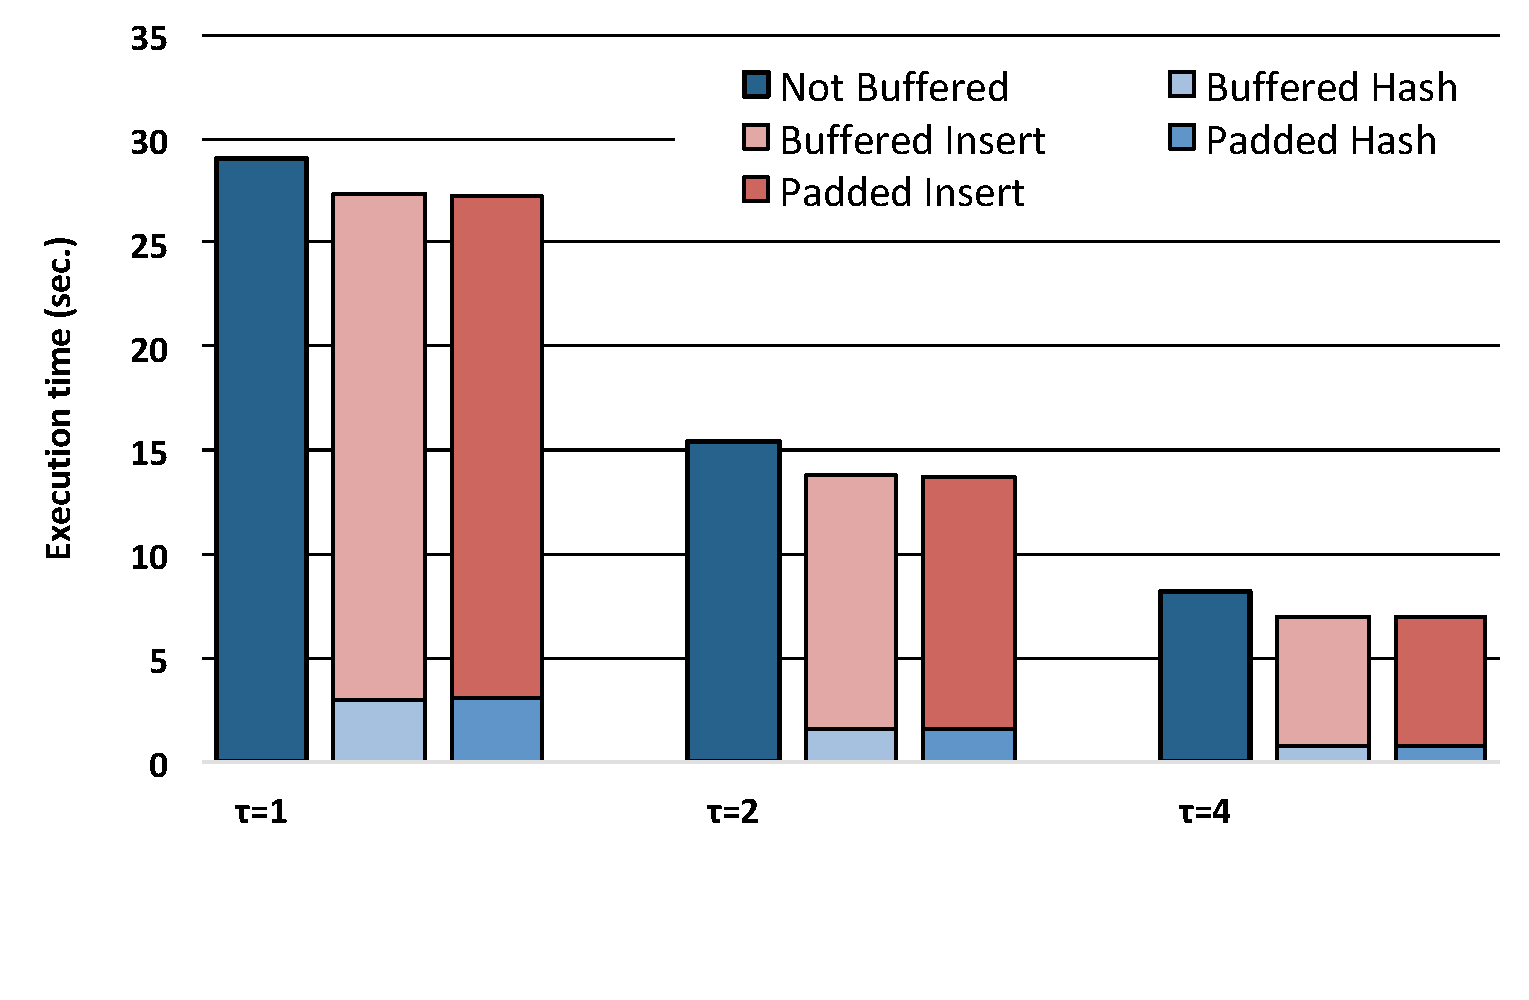
\includegraphics[width=\linewidth]{expfigs/small-rpi.pdf}
\caption{{\bf small} on {\bf Arch-2}}
\label{fig:8x211arch2}
\end{subfigure}
\begin{subfigure}[t]{0.43\textwidth}
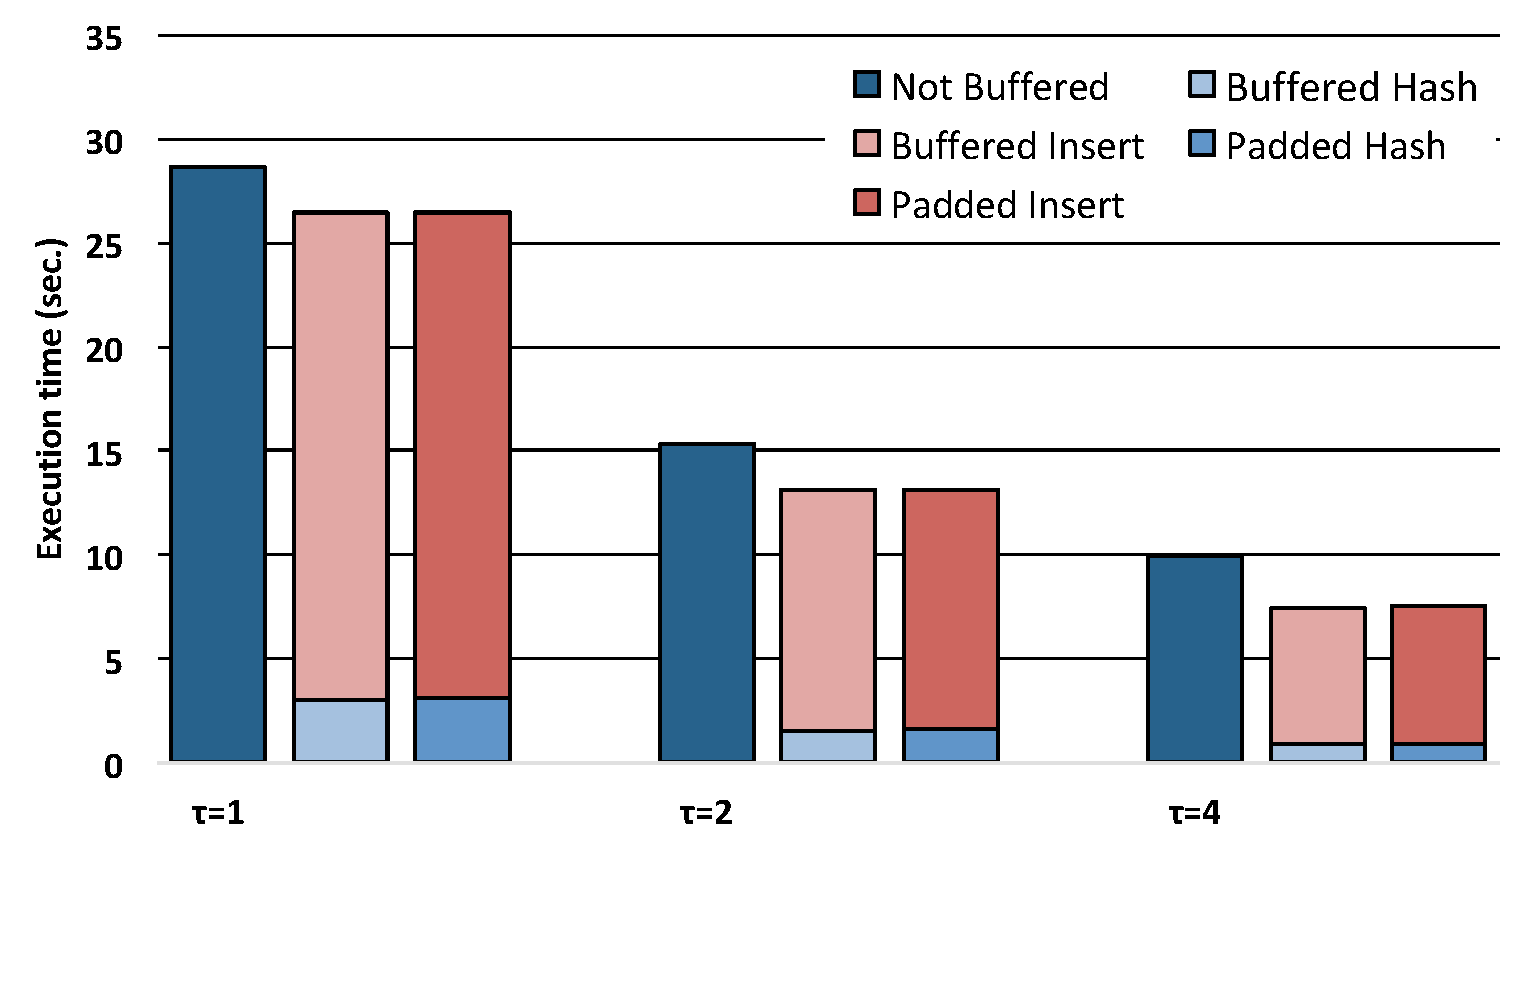
\includegraphics[width=\linewidth]{expfigs/large-rpi.pdf}
\caption{{\bf large} on {\bf Arch-2}}
\label{fig:8x2003arch2}
\end{subfigure}
\begin{subfigure}[t]{0.6\textwidth}
	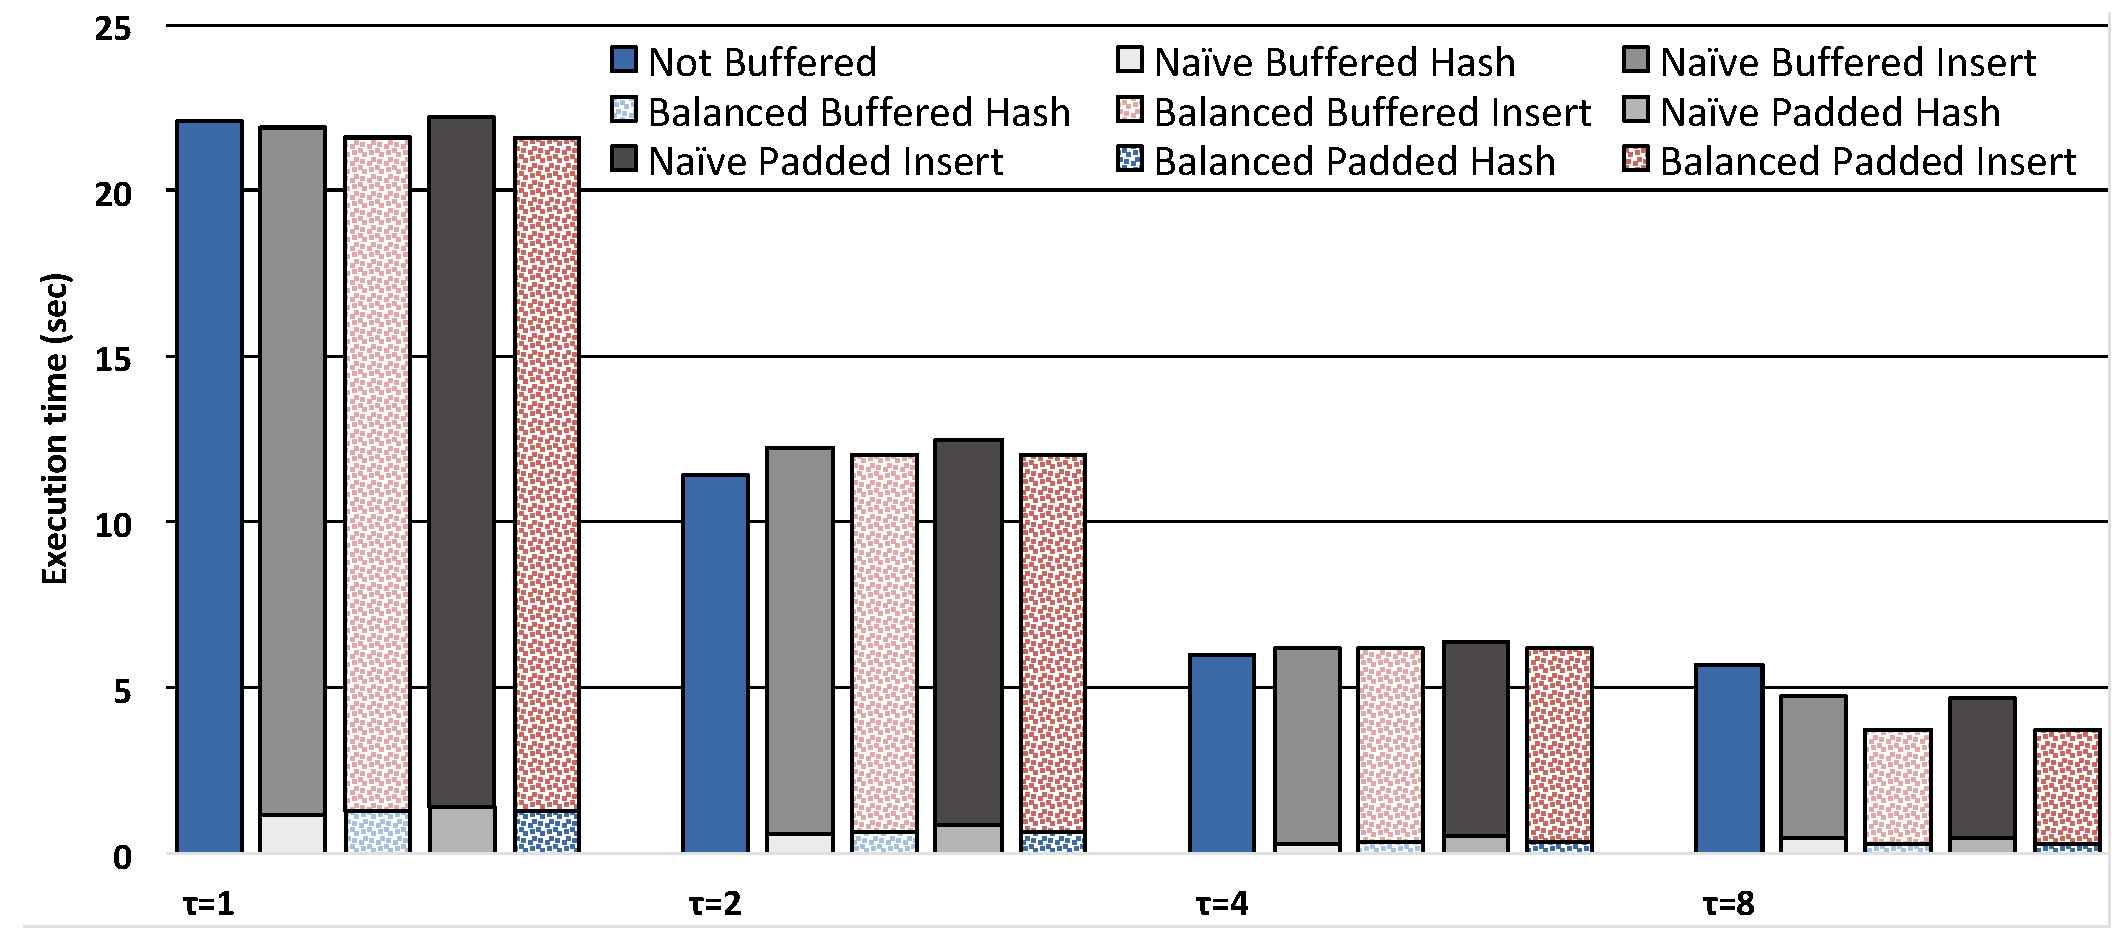
\includegraphics[width=\linewidth]{expfigs/small-odroid.pdf}
	\caption{{\bf small} on {\bf Arch-3}/{\bf{Arch-3++}}}
	\label{fig:8x211arch3}
\end{subfigure}
\begin{subfigure}[t]{0.6\textwidth}
	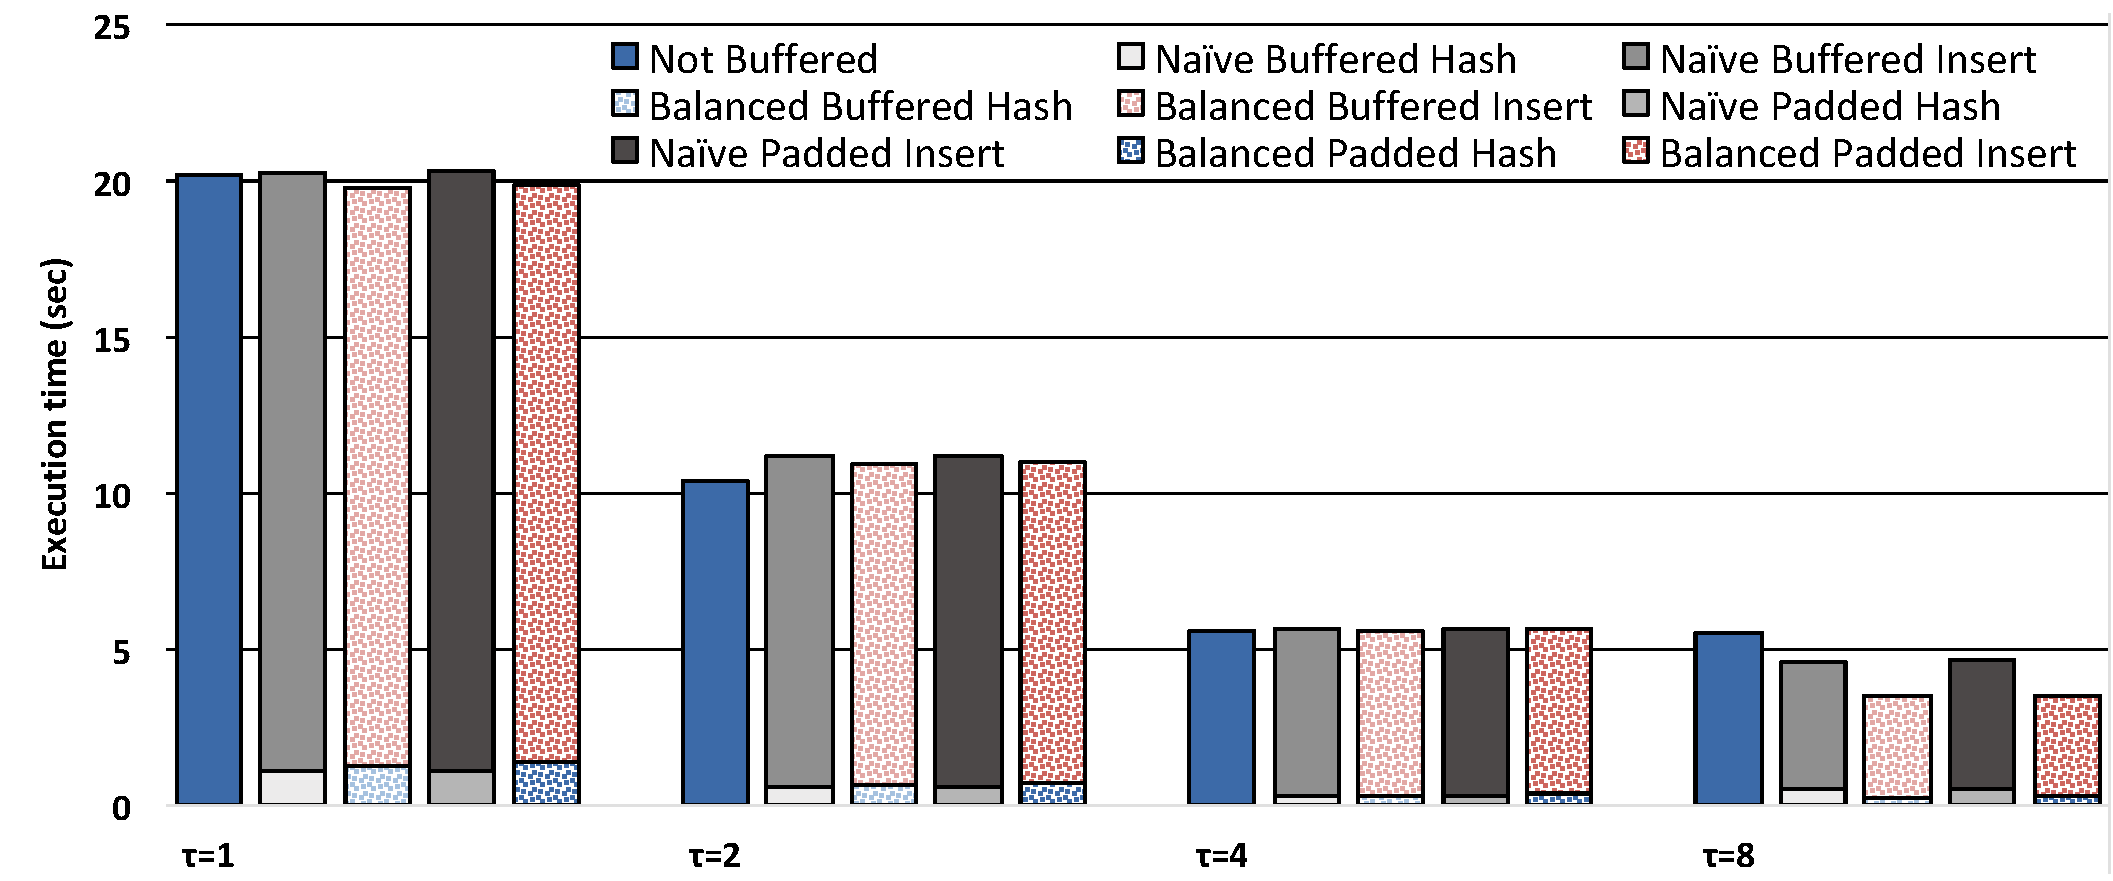
\includegraphics[width=\linewidth]{expfigs/large-odroid.pdf}
	\caption{{\bf large} on {\bf Arch-3}/{\bf{Arch-3++}}}
	\label{fig:8x2003arch3}
\end{subfigure}

\caption{Execution times (in seconds) for hashing and CMS update phase for single sketch experiments. The execution times for the naive parallel approach are omitted for {\bf Arch-1} since they are relatively much larger and deteriorate the visibility of the improvements.}
\label{fig:sum}
\end{figure*}

\subsection{Other optimizations and details}

In Algorithm~\ref{alg:cms_construct_par}, there is an implicit barrier between the first and second phases of the buffered construction. This barrier guarantees that the buffer is always full and ready to be processed at the beginning of the second phase. For the experiments given above, we removed this barrier on \textbf{Arch-1} and \textbf{Arch-2} but keep it on \textbf{Arch-3}. That is we implemented the buffered algorithms with OpenMPs {\tt nowait} directive on the first two architectures. This may have a negative impact on the accuracy; when threads do not wait for each other, there can exist an entry in the buffer which is not computed yet but being processed by a thread to update a counter. However, when $b$ is large, e.g., 1024, and cores are homogeneous, the probability of a thread using a buffer entry which is not correctly set is small. To analyze this option further, we performed two experiments; first, as Table~\ref{tbl:barrier} shows, removing the barrier usually has a positive impact on the performance on both \textbf{Arch-1} and \textbf{Arch-2}. However, it does not change the execution time on \textbf{Arch-3}. Hence, we opt to keep the barrier for this architecture.

To understand how the estimates change if the barrier is removed, we measured how much they deviate from a sequential execution~(which is the same as parallel executions with barriers). Figure~\ref{fig:err} show the absolute differences on the estimations when the barrier is kept or removed. The most frequent 1000 items are used for both charts in the figure. As the charts show, the differences are negligible on on \textbf{Arch-1} and \textbf{Arch-2} considering that the real frequencies are in the order of tens of thousands. Hemce, we opt to remove the barrier on these architectures. 
 
\begin{table*}[htbp]
	\centering
	{\def\arraystretch{1.0}
		\begin{tabular}{ccc||rrrr|rrrr}  
			&&                 & \multicolumn{4}{c|}{\textbf{Buffered Parallel + P}} & \multicolumn{4}{c}{\textbf{Buffered Parallel + PB}} \\
			&&                 &  $\tau$=2    & $\tau$=4    & $\tau$=8    & $\tau$=16  &  $\tau$=2   & $\tau$=4   & $\tau$=8   & $\tau$=16 \\ \hline
			
	\multicolumn{1}{l}{\multirow{6}{*}{{\rotatebox[origin=c]{90}{\textbf{Uniform}}}}}
			&\multirow{2}{*}{\textbf{Arch-1}} & \textbf{small}  &  43.5   & 22.8   & 13.0   & 10.6   &  43.8    & 23.5   & 13.5   & 11.1   \\
			&& \textbf{large} & 45.0   & 23.2   &   13.0 & 10.6   & 	44.0 &	23.7	& 13.6	& 11.1 \\ \cline{2-11}
			
			&\multirow{2}{*}{\textbf{Arch-2}} & \textbf{small}  &  13.8   & 6.9   &        &       &  14.3   & 10.4   &        &       \\
			&& \textbf{large} &    13.3     &       6.6 &        &       &          13.9    &     9.6   &        &   \\ \cline{2-11}
			
			&\multirow{2}{*}{\textbf{Arch-3++}} & \textbf{small}  &  12.2   & 6.2  & 3.9     &       &    12.2   & 6.2   &   3.9     &       \\
			&& \textbf{large} &    11.1     & 5.7 &  3.7      &       &          11.1   &     5.7   &   3.7     &   \\%\hline  
		\hline\hline
%			\multicolumn{1}{l}{\multirow{6}{*}{\textbf{Zipf 0.9}}}
%			&&&\multirow{2}{*}{\textbf{Arch-1}} & \textbf{small}  & 68.3    & 46.7   & 24.4   & 13.6   & 10.9   & 69.0    & 44.7    & 23.8   & 13.7   & 11.2   \\
%			&&&& \textbf{large} & 68.5    & 43.6   & 22.7   &   12.7 & 10.4   &  68.7 &	44.7 &	24.2	& 13.8	& 11.3 \\ \cline{4-15}
%			
%			&&&\multirow{2}{*}{\textbf{Arch-2}} & \textbf{small}  & 27.8    & 13.8   & 7.5   &        &       &  27.9    &  13.8   & 8.0   &        &       \\
%			&&&& \textbf{large} &  27.2      &   13.3     &       8.3 &        &       &     27.6   &     13.6    &     9.3   &        &   \\ \cline{4-15} 
%			
%			&&&\multirow{2}{*}{\textbf{Arch-3}} & \textbf{small}  & 21.8    & 12.1   & 6.2   & 3.8       &       &  21.8    &  12.2   & 6.2   &   3.8     &       \\
%			&&&& \textbf{large} &  20.6     &   11.1     & 5.7 &  3.6      &       &     20.6   &     11.1   &     5.7   &   3.7     &   \\ 
			
%			\hline  
\multicolumn{1}{l}{\multirow{6}{*}{{\rotatebox[origin=c]{90}{\textbf{Zipf 1.1}}}}}
			&\multirow{2}{*}{\textbf{Arch-1}} & \textbf{small}  &  43.5   & 22.9   & 13.0   & 10.6   & 45.6    & 24.6   & 14.2   & 11.5   \\
			&& \textbf{large} &  46.4   & 24.3   &   13.6 & 10.8   & 44.7 &	24.1	& 13.8	& 11.3 \\ \cline{2-11}
			
			&\multirow{2}{*}{\textbf{Arch-2}} & \textbf{small}  &  13.9   & 7.4   &        &       &    13.8   & 7.8   &        &       \\
			&& \textbf{large} &    13.3     &       8.1 &        &       &       13.5    &     9.3   &        &   \\ \cline{2-11}
			
			&\multirow{2}{*}{\textbf{Arch-3++}} & \textbf{small}  &  12.1   & 6.2   & 3.8     &       &   12.1   & 6.2   &   3.8     &       \\
			&& \textbf{large} &    11.1     & 5.7 &  3.6      &       &         11.2   &     5.8   &   3.7     &   \\  
			
			\hline  
			
\multicolumn{1}{l}{\multirow{6}{*}{{\rotatebox[origin=c]{90}{\textbf{Zipf 1.5}}}}}
			&\multirow{2}{*}{\textbf{Arch-1}} & \textbf{small}  & 44.6   & 23.5   & 13.1   & 10.6   &  44.3    & 24.2   & 13.8   & 11.4   \\
			&& \textbf{large} & 43.7   & 23.1   &   13.0 & 10.5   &  	44.2 &	23.6	& 13.6	& 11.0 \\ \cline{2-11}
			
			&\multirow{2}{*}{\textbf{Arch-2}} & \textbf{small}  &  13.7   & 7.0   &        &       &   13.7   & 7.0   &        &       \\
			&& \textbf{large} &   13.2     &       7.5 &        &       &          13.1    &     7.5   &        &   \\ \cline{2-11}
			
			&\multirow{2}{*}{\textbf{Arch-3++}} & \textbf{small}  & 12.1   & 6.2   & 3.8     &       &  12.0   & 6.1   &   3.8     &       \\
			&& \textbf{large} &     11.0     & 5.6 &  3.5      &       &          11.1   &     5.7   &   3.6     &   \\  
			
			\hline  
			
%				\multicolumn{1}{l}{\multirow{6}{*}{\textbf{Zipf 2}}}
%			&&&\multirow{2}{*}{\textbf{Arch-1}} & \textbf{small}  & 67.7    & 44.5   & 23.6   & 13.1   & 10.6   & 68.0    & 45.3    & 24.5   & 14.0   & 11.4   \\
%			&&&& \textbf{large} & 68.0    & 43.7   & 23.1   &   13.7 & 10.5   &  67.9 &	47.5 &	26.5	& 15.5	& 12.1 \\ \cline{4-15}
%			
%			&&&\multirow{2}{*}{\textbf{Arch-2}} & \textbf{small}  & 27.4    & 13.7   & 7.3   &        &       &  27.6    &  13.7   & 8.1   &        &       \\
%			&&&& \textbf{large} &  26.2      &   13.0     &       7.9 &        &       &     26.2    &     13.0    &     7.8   &        &   \\ \cline{4-15}
%			
%			&&&\multirow{2}{*}{\textbf{Arch-3}} & \textbf{small}  & 21.0    & 11.7   & 5.9   & 3.7     &       &  21.2    &  11.9   & 6.1   &   3.9     &       \\
%			&&&& \textbf{large} &  20.1     &   11.3     & 5.9 &  3.5      &       &     19.9   &     11.4   &     5.9   &   3.6     &   \\  
%			
%			\hline 

\multicolumn{1}{l}{\multirow{6}{*}{{\rotatebox[origin=c]{90}{\textbf{Zipf 3.0}}}}}
			&\multirow{2}{*}{\textbf{Arch-1}} & \textbf{small}  &  43.1   & 22.9  & 12.8   & 10.5   & 45.6    & 24.3   & 13.9   & 11.4   \\
			&& \textbf{large} &  44.4   & 23.1   &   13.1 & 11.2   &  	44.8 &	23.9	& 13.7	& 11.2 \\ \cline{2-11}
			
			&\multirow{2}{*}{\textbf{Arch-2}} & \textbf{small}  &  13.7   & 7.2   &        &       &   13.7   & 8.2   &        &       \\
			&& \textbf{large} &    13.1     &       7.4 &        &       &         13.1    &     7.8   &        &   \\ \cline{2-11}
			
			&\multirow{2}{*}{\textbf{Arch-3++}} & \textbf{small}  &  11.4   & 5.8  & 3.6     &       &   11.5   & 5.8   &   3.7     &       \\
			&& \textbf{large} &     11.1     & 5.5 &  3.4      &       &       11.1   &     5.8   &   3.5     &   \\
									
		\end{tabular}
		}



\caption{Impact of removing the barrier between the phases of buffered parallel execution on performance. The first set of the columns is the same with the last set of columns in Table~\ref{tbl:batch}. The values in the table are in seconds.}
\label{tbl:barrier}
\end{table*}

\begin{figure*}[htbp]
\begin{center}
\begin{subfigure}[t]{\textwidth}
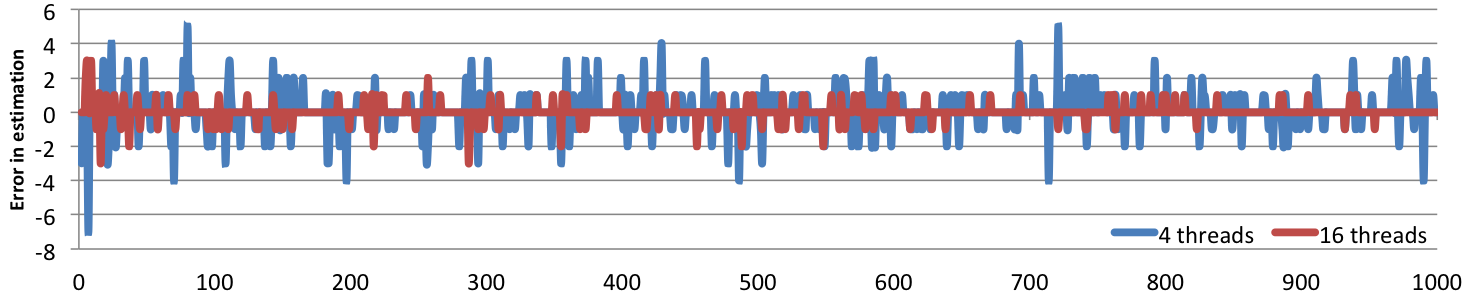
\includegraphics[width=\linewidth]{error1.png}
\caption{{\bf large} on {\bf Arch-1}}
\label{fig:err1}
\end{subfigure}
\end{center}

\begin{center}
\begin{subfigure}[t]{\textwidth}
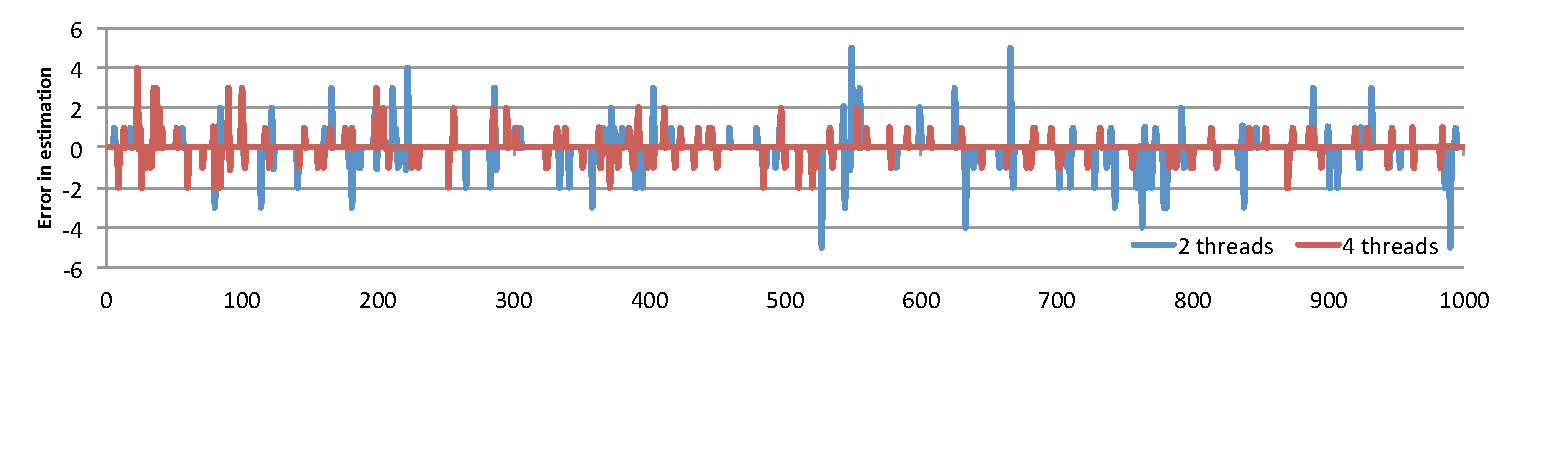
\includegraphics[width=\linewidth]{error2.pdf}
\caption{{\bf small} on {\bf Arch-2}}
\label{fig:err2}
\end{subfigure}
\end{center}

\caption{The difference between the frequency estimations of single and multithreaded executions of buffered parallel approach without the barrier. The charts show the differences for the top 1000 items for the {\bf large} sketch on {\bf Arch-1} and {\bf small} sketch on {\bf Arch-2}.}
\label{fig:err}
\end{figure*}


\section{Related Work}\label{sec:related}

CMS is proposed by Cormode and Muthukrishnan structure to summarize data streams~\cite{cormode2005} and it quickly became popular. They also suggest on sequential, parallel and hardware implementations of CMS~\cite{cormode2012} where the first parallel algorithm distributes rows to the threads so each thread computes the corresponding hash value. However, the hash computations are not merged as in our study. Another suggested algorithm is using multiple CMSs from different sub-streams and merge the results later.

Cafaro et al. propose an augmented frequency sketch for time-faded heavy hitters: recent items are considered to be more important~\cite{cafaro2016}. The authors extend this work via parallelization by dividing the stream into sub-streams and generating multiple sketches instead of a single one~\cite{cafaro2018}. When a query is issued, the result is computed using a reduce operation (as we did with multiple CMS tables in this study). There are studies in the literature employing synchronization primitives such as atomic operations for frequency counting~\cite{Das2009}. To the best of our knowledge, our work is the first cache-friendly, synchronization-free, single-table CMS algorithm specifically designed for limited-memory multicore architectures such as SBCs. Furthermore, it utilizes tabular hashing which is recently shown to provide good statistical properties and reported to be fast~\cite{thorup2017,Dahlgaard2017}. When multiple hashes on the same item are required, which is the case for many sketches, our table-merging technique will be useful for algorithms using tabular hashing. 

CMS has also been used as an underlying structure to design more advanced sketches. Recently, Roy et al. developed ASketch which filters high frequent items first and handles the remaining with a sketch such as CMS which they used for implementation~\cite{roy2016}. However, their parallelization depends on SPMD which stores multiple filters/sketches. Another advanced sketch employing multiple CMSs for parallelization is~\cite{Thomas2007}. If a single CMS sketch is necessary, e.g., to fit into the cache, our techniques can be employed to develop more advanced parallel sketches using table-based ones such as CMS or Count Sketch.

Overall, unlike most of the studies in the literature, we try to reduce the memory usage while staying scalable as
much as possible. Furthermore, to the best of our knowledge, this is the first study focusing on 
memory-restricted devices  such as SBCs for Count-Min Sketch.  

\section{Conclusion}\label{sec:con}

In this work, we investigated parallelization of Count-Min Sketch on three multicore architectures; a high-end server and two single board computers. We proposed three main techniques. The first one, merged tabulation, is useful when a single is item needs to be hashed multiple times and can be used for different sketches and other applications performing the same task. The second technique buffers the intermediate results to correctly synchronize the computation and regularize the memory accesses. The third one helps to utilize heterogeneous cores which is a recent trend on today's smaller devices. The experiments we performed show that all these techniques work for CMS construction on the architectures used for the experiments.

As a future work, we are planning to analyze the configuration options of the processors on single board computers such as how much data/instruction cache they use and how they handle coherency. Since sketches already incur inaccuracies, a freedom to have a little bit more can yield various optimizations. We also want to extend the architecture spectrum with other architectures such as FPGAs and other SBCs. We believe that similar techniques we develop here can also be used for other sketches. Finally, we are planning to work on different frequency sketches other than CMSs.


\bibliographystyle{ACM-Reference-Format}
\bibliography{sketch}
    
\end{document}
